% ============================================================================
% PhD Thesis Proposal
% Learning Automata Framework for Adaptive Kelp Forest Monitoring
% in British Columbia Coastal Waters
% Author: Ekaba Bisong
% University of Victoria
% ============================================================================

\documentclass[12pt,oneside]{book}

% ============================================================================
% PACKAGES
% ============================================================================
\usepackage[utf8]{inputenc}
\usepackage[T1]{fontenc}
\usepackage{lmodern}
\usepackage[margin=1in]{geometry}
\usepackage{setspace}
\usepackage{enumitem}
\usepackage{graphicx}
\usepackage{amsmath,amssymb,amsfonts}
\usepackage{algorithm}
\usepackage{algpseudocode}
\usepackage{booktabs}
\usepackage{multirow}
\usepackage{longtable}
\usepackage{array}
\usepackage{hyperref}
\usepackage{cleveref}
\usepackage{natbib}
\usepackage{xcolor}
\usepackage{tikz}
\usetikzlibrary{shapes,arrows,positioning,fit,calc}

% ============================================================================
% DOCUMENT SETTINGS
% ============================================================================
\hypersetup{
    colorlinks=true,
    linkcolor=blue,
    citecolor=blue,
    urlcolor=blue
}

\onehalfspacing

% Ensure all itemize lists use onehalfspacing
\setlist[itemize]{itemsep=0.1\baselineskip, parsep=0pt}
\setlist[enumerate]{itemsep=0.1\baselineskip, parsep=0pt}
% ============================================================================
% TITLE PAGE
% ============================================================================
\begin{document}

\begin{titlepage}
    \centering
    % \vspace*{0.5cm}

    {\Large\bfseries PhD Thesis Proposal\par}
    \vspace{1.5cm}

    {\LARGE\bfseries Learning Automata Framework for Adaptive Kelp Forest Monitoring in British Columbia Coastal Waters\par}

    \vspace{2cm}

    {\Large Ekaba Bisong\par}

    \vspace{1cm}

    {\large Department of Computer Science\\
    University of Victoria\\
    Victoria, British Columbia, Canada\par}

    \vspace{2cm}

    {\large Supervisory Committee:\par}
    \vspace{0.5cm}
    {\large Dr.\ Neil Ernst, Supervisor\\
    Dr.\ Maycira Costa, Committee Member\\
    Dr.\ Kevin Stanley, Committee Member\par}

    \vfill

    {\large \today\par}
\end{titlepage}

% ============================================================================
% ABSTRACT
% ============================================================================
\chapter*{Abstract}
\addcontentsline{toc}{chapter}{Abstract}

Kelp forests are among the most productive ecosystems on Earth, providing critical habitat, carbon sequestration, and coastal protection services. However, these ecosystems face immense threats from climate change stressors such as, marine heatwaves, and trophic cascades, thereby, causing a decline in kelp across British Columbia's coastline. Having an effective kelp forest management framework is critical for enhanced conservation and management efforts along British Columbia's 26,000+ km coastline especially given the heterogeneous environmental conditions that hampers real-time automated kelp monitoring systems.

This thesis proposes a Learning Automata (LA) framework for adaptive kelp forest monitoring that will address the following challenges: (1) adapting detection methods to diverse environmental conditions without extensive labeled data, (2) enabling effective monitoring across heterogeneous regions where single detection models have poor or significantly reduced performances, and (3) improving system performance using sparse, asynchronously-arriving validation labels. The proposed adaptive monitoring framework will incorporate three major components which include, a global policy learning mechanism using Linear Reward-Inaction ($L_{R-I}$) schemes to select optimal detection heuristics, a context-aware local adaptation system using memory-based similarity matching, and a sparse label handling module for delayed reward propagation.

We will evaluate the framework on the BC Bull Kelp dataset using Sentinel-2 satellite imagery. The evaluation will test adaptive monitoring performances across temporal, spatial, and environmental domains. The expected contributions of this thesis will include a novel application of learning automata to environmental monitoring, a methodology for handling sparse labels in operational systems, and a usable tool for kelp forest monitoring in BC coastal waters.

\tableofcontents

% ============================================================================
% CHAPTER 1: INTRODUCTION
% ============================================================================
\chapter{Introduction}
\label{ch:introduction}

\section{Background on Kelp Forest Ecology and Threats}
\label{sec:background}

Kelp forests is a productive and ecologically significant marine ecosystem that rivals tropical rainforests in their primary productivity and biodiversity support \citep{Steneck2002}. Kelp underwater forests are dominated by large brown macroalgae of the order \textit{``Laminariales''} forming complex three-dimensional habitats that support hundreds of associated species, from invertebrates to marine mammals. Along the Pacific coast of North America, two species dominate the canopy-forming kelp, they are, the giant kelp (\textit{Macrocystis pyrifera}) and bull kelp (\textit{Nereocystis luetkeana}), with bull kelp being the primary species in British Columbia's cooler waters \citep{Schroeder2020}.

British Columbia's coastline spans over 26,000 kilometers, and it represents one of the most extensive temperate kelp forest ecosystems globally \citep{Starko2024}. Kelp forests provide ecosystem services such as (1) habitat for commercially important fish and invertebrate species; (2) carbon sequestration through high rates of primary production; (3) coastal protection through wave attenuation; and (4) nutrient cycling that supports marine food webs \citep{Krumhansl2016}. For coastal First Nations communities, kelp forests hold deep cultural significance and have sustained traditional harvesting practices for millennia \citep{Kobluk2021, Dillehay2008, Erlandson2007, Turner2001}.

However, kelp forests worldwide are experiencing increasing pressure from multiple stressors. As an example, marine heatwaves, such as the 2014-2016 ``Blob'' event in the Northeast Pacific, have caused widespread kelp mortality through direct thermal stress \citep{Cavanaugh2019, MoraSoto2024}. In BC specifically, \citet{Starko2024} documented various concerning patterns of kelp forest decline across the province's 11 subregions, with some areas experiencing losses that exceed 70\% of its historical kelp coverage. These declines are a result of various interacting drivers. And they include, but not limited to: thermal stress in southern regions where sea surface temperatures regularly exceed the critical thresholds of 18--20$^\circ$C; trophic cascades in the northern regions where sea star wasting disease eliminated a critical kelp-protecting predator \textit{Pycnopodia helianthoides} that lead to an increase in the population of sea urchin and formation of urchin barrens \citep{Hamilton2021, Burt2018}.

The spatial variability of the factors contributing to kelp forest decline poses a significant challenge for monitoring systems.  In the southern Salish Sea, \citet{MoraSoto2024} delineated four distinct environmental clusters predicated on sea surface temperature, fetch, tidal currents, and suspended matter.  Each cluster showed different patterns of kelp growth and strength.  This means that detection methods that work well in one environment may not work well in another, so we need to come up with flexible methods that can work in different places.

\section{Problem Statement}
\label{sec:problem}

Tackling the problem of developing automated approaches to kelp forest monitoring is pertinent due to the scale and  heterogeneity of British Columbia's kelp forest ecosystems, and the various limitations faced by the current methods. As an example, satellite remote sensing provides the spatial coverage that is necessary for coastline-scale assessment, with sensors such as Sentinel-2 providing 10-meter resolution imagery every 5 days \citep{Gendall2023}. However, difficulty arises when translating this imagery into reliable kelp extent maps for several interconnected reasons.

Firstly, the spectral signature of floating kelp canopy varies with differing environmental conditions. Factors like water turbidity, sun glint, atmospheric conditions, tide height, and kelp physiological state all influence the detectability of kelp in satellite imagery \citep{Schroeder2020}. Whereby, methods that work well under ideal conditions such as calm water, low tide, and minimal cloud cover may fail to generalize when conditions deviate. The image quality scoring framework developed by \citet{Schroeder2020} show that a significant fraction of available imagery falls below reliability thresholds, thereby limiting the temporal frequency of monitoring.

Secondly, given the diversity of kelp forest environments along BC's coast, it is improbable that a single detection algorithm will perform optimally everywhere \citep{Starko2024, MoraSoto2024}. For example, bull kelp in exposed outer coastal environments will behave differently from bull kelp in protected inland waters \citep{Schroeder2019}. Further, kelp beds that are adjacent to sandy substrates have different spectral characteristics than those over rocky reef \citep{Timmer2022}. And the influence of adjacent land, river plumes, and industrial activities create site-specific detection challenges \citep{Schroeder2020}. Current approaches to kelp forest detection typically either: (a) apply a single method uniformly, accepting suboptimal performance in many areas; or (b) require extensive site-specific calibration that limits scalability \citep{Timmer2024}.

Thirdly, validation data for kelp detection is inherently sparse and asynchronously distributed \citep{CavanaughUAV2021}. Ground-truth surveys are expensive and logistically challenging in remote coastal areas \citep{Gendall2022drivers, Schroeder2019}, and cannot possibly keep up with the pace of satellite image acquisition. This issue creates a fundamental tension where methods need feedback to improve, but feedback arrives irregularly and with significant temporal lag relative to the imagery being validated. Traditional supervised learning approaches assume dense, contemporaneous labels that are unavailable in operational monitoring contexts.

These challenges motivate the need for a fundamentally different approach to kelp forest monitoring. And one that can adapt its detection strategy based on environmental context, learn from sparse, delayed feedback and continuously improve its detection accuracy without requiring extensive retraining or manual intervention.

\section{Research Objectives}
\label{sec:objectives}

The core objective of this research is to design a Learning Automata framework for adaptive kelp forest monitoring that will address the challenges of environmental heterogeneity and sparse validation feedback. The core objective will be expressed in the following ``sub''-objectives.

\begin{enumerate}
    \item \textbf{Designing a learning automata-based heuristic selection mechanism} that maintains a probability distribution across various detection methods (i.e. heuristics). It will update this distribution based on the performance it receives from the ``Environment'' thus enabling the system to converge toward optimal heuristic selection for given environmental conditions.

    \item \textbf{Developing a context-aware local adaptation component} that extracts environmental features from input imagery and uses memory-based similarity matching to blend global and local heuristic preferences, thereby enabling the system to generalize across the diverse environmental conditions present along BC's coastline.

    \item \textbf{Implementing a sparse label handling mechanism} that maintains a buffer of predictions yet to be validated. When the ground-truth labels eventually arrive, the delayed rewards are then calculated. This process enables the system to learn from irregular feedback patterns that are characteristic of operational monitoring.

    \item \textbf{Evaluating the framework} on the BC Bull Kelp dataset using Sentinel-2 imagery. The framework will assess the ability to monitor kelp forest ecosystems across temporal, spatial, and environmental domain shifts, with particular attention to performance in previously unseen conditions.

    \item \textbf{Exploring integration regimes} that incorporate Traditional Ecological Knowledge (TEK) from coastal First Nations communities into the monitoring framework. This integration must institute protocols that respect indigenous data sovereignty.
\end{enumerate}

\section{Research Questions}
\label{sec:research-questions}

This thesis addresses the following research questions that are organized by the specific challenges they target:

\subsection{Adaptation and Generalization}

\textbf{RQ1: How can we adapt kelp segmentation to diverse environmental conditions without extensive labeled data per region?}

This question addresses the fundamental tension between the need for site-specific optimization and the difficulty of obtaining sufficient labeled data for every environmental context along BC's coastline. The hypothesis is that a learning automata approach, which adapts based on sparse feedback rather than requiring dense supervision, can achieve effective adaptation with orders of magnitude fewer labels than conventional approaches.

\textbf{RQ2: Can adaptive selection of detection methods enable effective monitoring across heterogeneous regions where single models fail?}

This question examines whether dynamic selection among a pool of diverse heuristics outperforms any fixed approach when applied across the range of environmental conditions present in BC waters. The hypothesis is built on the idea that different heuristics will exhibit complementary strengths across conditions, and that adaptive selection can exploit this complementarity to achieve robust performance.

\subsection{Learning from Sparse Feedback}

\textbf{RQ3: How can a monitoring system improve its performance during deployment using sparse, asynchronously-arriving validation labels?}

This question addresses the operational reality that ground-truth validation arrives irregularly, perhaps within days or even months after image acquisition. The hypothesis is that a properly designed sparse label handling mechanism can propagate delayed rewards effectively, thereby enabling continuous improvement despite irregular feedback.

\subsection{Knowledge Integration}

\textbf{RQ4: How can Traditional Ecological Knowledge from coastal First Nations be integrated into automated kelp forest monitoring?}

This question acknowledges that quantitative satellite-based monitoring represents only one way of knowing about kelp forest dynamics. The hypothesis is that indigenous knowledge systems offer complementary temporal depth, spatial resolution, and contextual understanding that can enhance automated monitoring when integrated through appropriate protocols that respect indigenous data sovereignty \citep{Reid2021, Proulx2021}.

\section{Scope and Delimitations}
\label{sec:scope}

This research will focus specifically on:

\begin{itemize}
    \item \textbf{Geographic scope:} British Columbia coastal waters, with experimental validation on representative subregions that span the environmental gradients that are present along the coast (e.g., exposed outer coast, protected inland waters, areas with and without sea otter populations).

    \item \textbf{Species scope:} Canopy-forming kelp, primarily bull kelp (\textit{Nereocystis luetkeana}) with potential extension to giant kelp (\textit{Macrocystis pyrifera}) in southern areas where both species occur.

    \item \textbf{Sensor scope:} We will use Sentinel-2 multispectral imagery as the primary data source. The reason for this choice is its combination of spatial resolution (10m), temporal frequency (5 days), spectral bands (including red-edge), and free availability.

    \item \textbf{Temporal scope:} We will use Sentinel-2 archive for BC waters from 2017--2024. The aim is to have sufficient temporal depth to assess adaptation across interannual variability and climate anomalies.

    \item \textbf{Methodological scope:} Learning automata with discrete heuristic selection. Further, continuous action learning automata and hierarchical structures are identified as potential extensions.
\end{itemize}

The following aspects are explicitly outside the scope of this research:

\begin{itemize}
    \item Subsurface kelp monitoring (the focus is on floating canopy detectable by optical sensors)
    \item Real-time operational deployment (the focus is on developing and validating the methodology)
    \item Comprehensive integration with management decision systems
    \item Detailed physiological or ecological modeling of kelp dynamics
\end{itemize}

\section{Significance of the Study}
\label{sec:significance}

This research contributes to multiple domains:

\textbf{Scientific Contributions:} The proposed framework represents a novel application of learning automata theory to environmental monitoring and to address the specific challenges of remote sensing-based ecosystem assessment. The integration of context-aware adaptation using generalized learning automata principles addresses fundamental questions about how intelligent systems can adapt to heterogeneous environments with minimal supervision.

\textbf{Methodological Contributions:} While sparse and delayed feedback is recognized as a fundamental challenge in reinforcement learning \citep{SuttonBarto2018}, its application to operational environmental monitoring systems where ground-truth validation may arrive weeks to months after predictions remains underexplored. The proposed approach of delayed reward propagation through temporal buffers addresses this domain-specific challenge.

\textbf{Practical Contributions:} BC's kelp forests face documented and ongoing decline \citep{Starko2024}, yet comprehensive monitoring remains challenging due to the scale of the coastline (over 26,000 km) and the heterogeneity of environmental conditions \citep{MoraSoto2024}. An adaptive monitoring system could provide the spatial coverage and temporal frequency needed to inform conservation and management decisions such as identifying areas of concern and tracking the effectiveness of interventions.

\textbf{Broader Impact:} The methodological advances we will develop for kelp monitoring will have potential applications to other spatially extensive, environmentally heterogeneous monitoring challenges such as seagrass meadows, coral reefs and terrestrial forests. The framework's emphasis on adaptation with sparse feedback is particularly relevant for deploying monitoring systems in data-scarce environments.

% I started using Humanizer here.

% ============================================================================
% CHAPTER 2: LITERATURE REVIEW
% ============================================================================
\chapter{Literature Review}
\label{ch:literature}

\section{Kelp Forest Ecology and Dynamics}
\label{sec:lit-kelp-ecology}

\subsection{Structure and Function of Kelp Forest Ecosystems}
\label{subsec:structure-function}

Kelp forests are very productive ecosystems, with net primary production of 500 to over 1,000 g C m$^{-2}$ year$^{-1}$ in dense stands \citep{Steneck2002, Mann1973}. Kelp-derived organic matter fuels complex food webs via herbivory, detrital processing and dissolved organic carbon export \citep{Duggins1989, Graham2004}. Predators have a strong top-down control over these food webs, with effects that propagate through multiple trophic levels \citep{Halpern2006}. The three-dimensional structure of kelp canopy, stipe, and holdfast offers habitat at many scales, from microscopic communities colonizing the surface of the kelp to large predators hunting in the kelp forests \citep{Dayton1985a, Teagle2017}. Kelp population dynamics are determined by oceanographic climate operating at temporal and spatial scales \citep{Dayton1999} and global assessments suggest that kelp forests are undergoing widespread changes with regional variability far exceeding global averages \citep{Krumhansl2016, Wernberg2019}.

In British Columbia two canopy-forming species predominate. Bull kelp (\textit{Nereocystis luetkeana}) is the dominant species, with a single large pneumatocyst bearing a canopy of blades up to more than 30 meters from the seafloor to the surface. Unlike the perennial giant kelp of California, bull kelp is an annual species that recruits from spores released in autumn and deteriorates after reproducing \citep{Springer2007}. This annual life history makes bull kelp populations especially sensitive to environmental conditions during the critical spring to summer growth period. \citet{Schroeder2019} provide a very thorough review of passive remote sensing methods for mapping bull kelp, including application of these methods through a case study in British Columbia.

Giant kelp (\textit{Macrocystis pyrifera}) is found in southern British Columbia, especially the Strait of Juan de Fuca and the outer coast of Vancouver Island, where water temperatures are within the thermal tolerance of giant kelp. Giant kelp is perennial and can persist for several years, offering more temporally stable structure than bull kelp but showing greater sensitivity to thermal stress during warm-water anomalies \citep{Cavanaugh2019}. \citet{ BellSiegel2022} showed that nutrient availability and senescence spatially structure giant kelp dynamics with remote sensing showing how physiological stress propagates through kelp forest canopies.

\subsection{Threats and Stressors}
\label{subsec:threats}

Kelp forests are experiencing a range of interacting stressors that can lead to sudden state changes. \citet{Starko2024} present the most comprehensive study of the dynamics of BC kelp forests, including variable patterns of change across the BC coastline:

\textbf{Thermal stress:} Marine heatwaves, especially the 2014--2016 ``Blob'' event, led to extensive kelp mortality by direct physiological stress \citep{Bond2015, DiLorenzoMantua2016, Smale2019}. In the southern Salish Sea, summer sea surface temperatures regularly exceed the 18--20$^\circ$C thresholds beyond which kelp photosynthesis and growth are impaired \citep{MoraSoto2024}. \citet{Berry2021} published a 63\% decline in bull kelp extent in South Puget Sound over 145 years, with losses concentrated along wave-sheltered shorelines with elevated temperatures. \citet{Schroeder2020} published a 48.6\% decline in kelp extent from 2015 to 2017 The Kelpwatch platform developed by \citet{Bell2023} showed that 18.6\% of regional sites throughout California and Mexico showed significant long-term trends, with variable recovery patterns after marine heatwaves. In northern California, \citet{RogersBennett2019} observed catastrophic losses of greater than 90\% of bull kelp canopy following the marine heatwave, with the persistent urchin barrens preventing recovery \citep{McPherson2021}. The delay between thermal stress and population decline (roughly one year) is a complicating feature but is consistent with impacts on reproduction and juvenile survival.

\textbf{Trophic cascades:} In northern BC, declines in kelp were observed despite the lower temperatures that should have been favourable for kelp growth. The explanation is the 2013-2017 sea star wasting disease epidemic that effectively extirpated the sunflower sea star (\textit{Pycnopodia helianthoides}) throughout its range \citep{Hamilton2021, Harvell2019}. Sunflower stars were the main predator of sea urchins in many places; their removal caused explosive urchin population growth and subsequent overgrazing of kelp, a phenomenon called ``trophic cascade to urchin barrens'' \citep{Burt2018, EstesDuggins1995, Ling2015}. This trophic cascade mechanism has been reported worldwide as a major cause of kelp forest collapse \citep{Ling2009, EstesPalmisano1974}.

\textbf{Wave exposure:} Physical disturbance from storm waves directly removes kelp biomass, but moderate wave action can also be beneficial to kelp by limiting urchin grazing (urchins are dislodged by wave surge) and increased nutrient delivery due to water mixing. The relationship between wave exposure and kelp persistence is therefore non-linear and context-dependent \citep{Starko2024}.

\subsection{Resilience and Recovery}
\label{subsec:resilience}

Kelp forest resilience differs markedly along the BC coastline, with different mechanisms providing stability in different regions. \citet{MoraSoto2024} identified four environmental clusters in the southern Salish Sea, each with different patterns of resilience:

\begin{enumerate}
    \item \textbf{Cold, exposed sites} (e.g., outer coast of southern Vancouver Island): High resilience with favorable thermal conditions that buffer against impacts of heatwaves.

    \item \textbf{Semi-sheltered sites}: Moderate resilience, with potential for reduced wave stress and sufficient water mixing.

    \item \textbf{Strait of Georgia sites}: Low resilience, experiencing the most extreme temperatures and variability in kelp persistence.

    \item \textbf{Warm, protected sites}: Low overall kelp occurrence; could exhibit resilience in areas with local conditions that form thermal refugia.
\end{enumerate}

At a provincial scale, \citet{Starko2024} found that areas with sea otter populations were more stable, which highlights the importance of top-down trophic control. Whereas sea otters were present, urchin grazing was suppressed regardless of sunflower star status, providing functional redundancy in the predator guild.

\subsection{Phase Shifts and Tipping Points}
\label{subsec:phase-shifts}

The shift from kelp forest to urchin barren is an example of a classic ecological phase shift - a rapid reorganization of ecosystem state that may be difficult to reverse \citep{Holling1973, Steneck2002, Steneck2008, FilbeeDexter2018}. \citet{FilbeeDexter2014} presented a comprehensive review of sea urchin barrens as alternative stable states of collapsed kelp ecosystems. \citet{Wilman2021} created a mathematical model of the predator-urchin-kelp ecosystem that shows that pulse disturbances can trigger shifts between equilibria and there is hysteresis, meaning catastrophic shifts are imperfectly reversible. \citet{Wernberg2016} reported a climate-driven regime shift in Western Australia where a marine heatwave led to a 100~km poleward contraction of kelp forests. Once urchins reach high densities, they can persist in a ``barren'' condition even when conditions are otherwise favorable for kelp recovery, leading to hysteresis in the system dynamics \citep{Ling2015}. Despite regional collapse, some refugia remain where kelp is able to survive despite unfavorable regional conditions \citep{CavanaughKC2023}, making fine-scale monitoring important for identifying and protecting such areas.

Understanding and detecting such phase shifts is an important motivation for adaptive monitoring systems. Traditional monitoring approaches, assuming gradual, linear change, may not be able to detect leading indicators of imminent state shifts \citep{Reed2016} while adaptive systems that track regime specific dynamics could offer early warning of critical transitions. \citet{Reed2015} emphasized the value of broad temporal and spatial perspectives for understanding the dynamics of kelp forest ecosystems, demonstrating through the Santa Barbara Coastal LTER that short term, small scale studies often fail to capture the drivers of ecosystem change. Long-term monitoring datasets are required to understand variability in kelp forests at temporal scales \citep{Malone2022, Pfister2018}. \citet{Krumhansl2024} showed that kelp forests in Nova Scotia exhibited resilience despite rapid ocean warming, with shifts in community composition in favor of warm-tolerant species while maintaining stability in overall kelp abundance.

\subsection{Geographic Variability and Implications for Monitoring}
\label{subsec:geographic-variability}

A critical challenge for kelp forest monitoring systems is the large geographical variability in kelp species, environmental conditions and ecosystem dynamics in different coastal regions. This variability has profound implications for the design of detection algorithms, and it raises the possibility that algorithms that are adaptive and tailored to individual contexts may be more effective than universal models.

\textbf{Scale-dependent processes:} \citet{Marzinelli2015} showed that processes structuring kelp assemblages at small scales (10--100 m) did not generalize well to larger scales (100--1,000 km), owing to intrinsic spatial and temporal variability in natural systems. \citet{UnderwoodPetraitis1993} formalized this challenge, arguing that if we compare local processes in different locations, we have to explicitly consider the effect of scale on detecting patterns. This fundamental ecological insight suggests that monitoring algorithms that are optimized for one spatial or temporal scale may be poor at others.

\textbf{Regional kelp communities:} Different geographical regions support different kelp species assemblages with different morphologies and spectral signatures. In the Arctic, \citet{Bischof2019} described the effects of unique Arctic stressors such as UV radiation, ice cover dynamics, and progressive ``Atlantification'' on \textit{Laminaria solidungula} and other kelp species in Kongsfjorden, fundamentally different from temperate kelp forests. Australian temperate reefs are dominated by \textit{Ecklonia radiata}, with kelp cover increasing with latitude, but being highly variable at smaller scales \citep{Marzinelli2015, ConnellIrving2008}. In the northeastern Atlantic, \citet{Voerman2013} documented climate driven changes in NW Spain kelp communities, which included a decline of almost 1,400 ha and shifts in species composition favoring warm tolerant taxa-patterns distinct to those seen in the Pacific kelp. On the Atlantic coast of Canada, \citet{JohnsonMann1988} showed that \textit{Laminaria longicruris} shows multiple patterns of adaptation allowing dominance in habitats with varying nutrient stress, and various disturbance levels, and \citet{SimmsDubois2001} developed satellite remote sensing methods for mapping submerged kelp beds in this region. In glacially-impacted environments, \citet{Huovinen2020} showed that mapping of kelp in Patagonian fjords will need to consider unique water optical properties affected by glacier runoff.

\textbf{Implications for detection systems:} These geographic variations suggest that: (1) detection algorithms trained on data from one region may not transfer effectively to others; (2) spectral signatures of kelp canopy vary with species composition, water properties and environmental conditions \citep{Turner2003}; and (3) the optimal detection heuristic for a given image tile is dependent on its geographic and environmental context. \citet{Wernberg2012} reviewed a decade of climate change experiments on marine organisms and found that small-scale manipulative experiments often fail to predict large-scale responses, reinforcing the need for monitoring approaches that can adapt across scales and contexts.

This geographical variability represents the fundamental motivation for the adaptive context-aware framework proposed in this thesis. Instead of attempting to find a single universal detection model, the Learning Automata approach learns to choose the optimal heuristic for each environmental context, with the assumption that such adaptive selection will perform better than any single fixed approach. \citet{Yong2005} showed this principle in general image segmentation, where learning-based algorithm selection based on image features to predict optimal segmentation methods achieved 85\% accuracy in choosing the best algorithm - a compelling precedent for adaptive heuristic selection for kelp detection.

\section{Monitoring Techniques in Kelp Forests}
\label{sec:lit-monitoring}

\subsection{Traditional Survey Techniques}
\label{subsec:traditional-surveys}

Traditional kelp monitoring is based on direct observation using methods including:

\textbf{Shoreline surveys:} Walking or kayaking along coastlines during low tide and mapping visible kelp beds. While offering high spatial resolution and species identification, these approaches are labor-intensive, limited by access, and can only be used to cover small portions of large coastlines.

\textbf{SCUBA transects:} Underwater surveys recording kelp density and size structure, and associated fauna, along fixed transects. These supply the most detailed ecological information, but are very limited in spatial information and require specialized personnel.

\textbf{Aerial photography:} Photographs taken by fixed-wing aircraft or helicopters, which take oblique or vertical photographs. The ShoreZone project has amassed a large amount of oblique shoreline imagery for BC, a great historical baseline \citep{Starko2024}. However, aerial surveys are costly, dependent on the weather, and are only performed once every 10--15 years.

\subsection{Remote Sensing Methods}
\label{subsec:remote-sensing}

Satellite remote sensing provides the spatial coverage required for coastline-scale monitoring, with a number of platforms having relevant capabilities \citep{Bennion2019, Cavanaugh2021}:

\textbf{Landsat (30m resolution):} The longest continuous record of Earth observation, with archives extending to the 1970s. \citet{Cavanaugh2010} demonstrated scaling of giant kelp field measurements to regional scales using Landsat, while \citet{Cavanaugh2011} showed environmental controls of kelp biomass through 25 years of Landsat observations in the Santa Barbara Channel. \citet{MoraSoto2024} used Landsat for long-term sentinel site analysis at Ella Beach, BC spanning 50 years. \citet{Bell2020} reconstructed three decades of California giant kelp variability from Landsat, demonstrating the value of long-term satellite archives \citep{Finger2021, Hamilton2020}. \citet{Houskeeper2022} demonstrated automated satellite detection of giant kelp at the Falkland Islands using spectral unmixing algorithms. \citet{Nijland2019} developed a Google Earth Engine \citep{Gorelick2017} tool for automated Landsat-based kelp detection specifically designed for BC's complex coastline, achieving 80\% overall accuracy while quantifying tidal effects on kelp extent detection.

\textbf{Sentinel-2 (10m resolution):} The European Space Agency's optical sensor provides improved spatial resolution, more spectral bands (including red-edge bands sensitive to vegetation), and 5-day revisit time through the twin-satellite constellation. \citet{Gendall2023} developed a multi-satellite mapping framework incorporating Sentinel-2 for floating kelp canopy detection. \citet{MoraSoto2020} created a high-resolution global map of giant kelp forests using Sentinel-2, providing algorithm thresholds applicable across hemispheres. \citet{Timmer2022} compared red-edge and near-infrared wavelengths for detecting submerged kelp canopy in BC waters. \citet{Timmer2024} demonstrated the importance of integrating tides, currents, and species-level morphology when mapping kelp from remote sensing imagery, showing that environmental conditions during image acquisition significantly affect detection accuracy. \citet{StPierre2020} established a framework for kelp-bed mapping using supervised classification of satellite imagery, achieving 89\% overall accuracy for submerged kelp detection.

\textbf{High-resolution commercial sensors:} WorldView-2/3 (1.2--2.6m) and CubeSat constellations like PlanetScope (3m) provide fine spatial resolution. \citet{Schroeder2020} used WorldView imagery for detailed kelp mapping in the Cowichan Bay area, achieving 86.9\% overall accuracy. \citet{CavanaughKC2023} demonstrated PlanetScope for detecting fine-scale kelp refugia that coarser resolution sensors miss.

\textbf{Unoccupied Aerial Vehicles (UAVs):} UAVs offer sub-meter resolution for local-scale monitoring and restoration assessment. \citet{Saccomanno2023} developed methods for mapping emergent kelp canopy following ecological regime shifts, demonstrating the complementary role of UAVs alongside satellite data. \citet{CavanaughUAV2021} developed an automated method for mapping giant kelp canopy dynamics from UAV imagery, achieving 93\% accuracy with multispectral sensors and quantifying the effects of tides and currents on visible kelp canopy.

\subsection{Classification Indices and Methodology}
\label{subsec:classification-methods}

Several spectral indices have been successful for the detection of kelp:

\textbf{NDVI (Normalized Difference Vegetation Index):} Standard vegetation index based on red and near-infrared bands. Effective for separating kelp from open water and can confuse kelp with other floating vegetation or surface algae.

\textbf{GNDVI (Green Normalized Difference Vegetation Index):} In GNDVI, green is used instead of red, which allows for greater sensitivity to chlorophyll content. \citet{Schroeder2020} found GNDVI complementary to NDVI for kelp classification.

\textbf{FAI (Floating Algae Index):} Specifically designed for floating vegetation, FAI makes use of the red-edge spectral region in which submerged and floating vegetation are different \citep{Gendall2023}.

\textbf{NDWI (Normalized Difference Water Index):} Useful for separating water from other surfaces but usually used as a mask rather than directly for kelp detection.

\subsection{Machine Learning for Kelp Detection}
\label{subsec:ml-kelp}

Recent advances in machine learning have enabled more sophisticated kelp detection approaches \citep{Ma2019}:

\textbf{Random Forest and other ensemble methods:} Combining multiple spectral features through decision tree ensembles has shown strong performance for kelp classification. \citet{Ganaie2022} provide a comprehensive review of ensemble deep learning approaches, while \citet{Savargiv2021} demonstrated learning automata integration with Random Forest for improved classifier selection. \citet{TonionPirotti2022} achieved over 98\% overall accuracy using Random Forest for seaweed detection along the Irish coast, demonstrating the potential for ML-based monitoring when sufficient training data is available.

\textbf{Convolutional Neural Networks:} Deep learning approaches, particularly U-Net architectures for semantic segmentation, have achieved state-of-the-art performance in kelp detection when sufficient training data is available \citep{Ma2019, Bai2023}. \citet{Marquez2022} demonstrated Mask R-CNN for giant kelp forest mapping from Landsat imagery, achieving Jaccard indices of 0.87 and enabling reconstruction of 32-year time series with reduced human effort. \citet{Mahmood2020} developed hierarchical classification using deep residual features for kelp classification from AUV imagery, achieving 90\% accuracy while demonstrating the value of hierarchical classification approaches over flat classification. Most recently, \citet{Nasios2025} demonstrated that combining Vision Transformers with ConvNeXt models and crowdsourced labels achieves high kelp detection accuracy from Landsat imagery, identifying approximately three out of four kelp canopy pixels.

\textbf{Reinforcement Learning:} Deep reinforcement learning approaches are emerging for conservation decision-making \citep{Lapeyrolerie2022}, offering potential for adaptive monitoring systems that learn optimal strategies through interaction with the environment. \citet{Lindkvist2017} demonstrated that computational adaptive management using reinforcement learning can find optimal strategies for sustainable resource management during environmental change, with results showing that strategies optimized for declining growth rates are robust to fluctuating or increasing growth.

\textbf{Limitations:} These methods require substantial labeled training data and may not generalize well across environmental conditions not represented in training. The transfer learning challenge that adapts a model trained in one region or time period to new conditions remains an active research area. \citet{BeasLuna2020} demonstrated that kelp forest responses to climate vary geographically, highlighting the need for adaptive approaches that account for regional heterogeneity.

\section{Learning Automata Theory}
\label{sec:lit-la}

\subsection{Historical Development and Foundations}
\label{subsec:la-foundations}

Learning Automata (LA) emerged in the Soviet Union in the 1960s through the pioneering work of Tsetlin \citep{Tsetlin1961}, who proposed computational adaptive schemes for learning optimal actions in stochastic environments. The field evolved out of the combination of automata theory, stochastic processes, and behavioral psychology - especially conditioning and associative learning theories formalized computationally by \citet{BushMosteller1955}. LA share conceptual interfaces with reinforcement learning, multiagent systems and control theory, but provide different theoretical guarantees that are particularly relevant to decision-making under uncertainty \citep{Narendra1989, ThathacharSastry2002, Bisong2018}.

The LA model works in a feedback loop between the automaton (decision-maker) and an unknown environment. This formulation is especially well suited for situations where little or no information is known \textit{a priori} about environmental response characteristics. This LA framework resembles kelp monitoring very closely, where detection algorithm performance varies unpredictably across environmental situations.

\subsection{Mathematical Framework}
\label{subsec:la-math-framework}

The LA framework consists of two interacting components: the \textbf{Environment} and the \textbf{Automaton} \citep{Narendra1989, Bisong2018}.

\textbf{Environment.} The environment is an abstract stochastic medium represented as a triple $E = \{\alpha, c, \beta\}$ where:
\begin{itemize}
    \item $\alpha = \{\alpha_1, \alpha_2, \ldots, \alpha_r\}$ is the set of $r$ input actions
    \item $\beta$ is the feedback response. Three models exist:
    \begin{itemize}
        \item \textit{P-model:} Binary response $\beta \in \{0, 1\}$ (reward/penalty)
        \item \textit{Q-model:} Finite discrete values in $[0,1]$
        \item \textit{S-model:} Continuous random variable in $[0,1]$
    \end{itemize}
    \item $c = \{c_1, c_2, \ldots, c_r\}$ are penalty probabilities where $c_i = P(\beta(n) = 1 \mid \alpha(n) = \alpha_i)$
\end{itemize}
The S-model is particularly relevant to the proposed framework, as performance metrics such as F1-score and IoU are continuous values in $[0,1]$ that naturally serve as feedback signals.

\textbf{Automaton.} The automaton is described as a quintuple $A = \{\Phi, \alpha, \beta, F(\cdot,\cdot), G(\cdot,\cdot)\}$ where:
\begin{itemize}
    \item $\Phi = \{\phi_1, \phi_2, \ldots, \phi_s\}$ is the finite set of internal states
    \item $\alpha$ and $\beta$ are as defined for the environment
    \item $F: \Phi \times \beta \rightarrow \Phi$ is the state transition function: $\phi(n+1) = F[\phi(n), \beta(n)]$
    \item $G: \Phi \rightarrow \alpha$ is the output mapping that determines action selection
\end{itemize}

\subsection{Performance Criteria and Optimality}
\label{subsec:la-performance}

The quality of an LA is evaluated by comparing its expected penalty $M(n) = E[\beta(n)|P(n)] = \sum_{i=1}^{r} c_i p_i(n)$ against a pure-chance automaton $M_0 = \frac{1}{r}\sum_{i=1}^{r} c_i$ that selects actions uniformly at random \citep{Narendra1989}. The following performance criteria are established:

\begin{itemize}
    \item \textbf{Expedient:} $\lim_{n\to\infty} E[M(n)] < M_0$ (better than pure chance)
    \item \textbf{Optimal:} $\lim_{n\to\infty} E[M(n)] = c_\ell$ where $c_\ell = \min_i c_i$
    \item \textbf{$\epsilon$-optimal:} $\lim_{n\to\infty} E[M(n)] < c_\ell + \epsilon$ for arbitrary $\epsilon > 0$
    \item \textbf{Absolutely Expedient:} $E[M(n+1)|P(n)] < M(n)$ (continually decreasing)
\end{itemize}

These criteria provide theoretical guarantees that are essential for the proposed framework: an $\epsilon$-optimal LA will asymptotically select the best-performing heuristic with arbitrarily high probability.

\subsection{Fixed and Variable Structure Automata}
\label{subsec:fssa-vssa}

LA are categorized into two families based on their transition characteristics \citep{Narendra1989, Bisong2018}:

\textbf{Fixed Structure Stochastic Automata (FSSA).} In FSSA, state transitions are deterministic given the current state and feedback. The Tsetlin automaton $L_{2N,2}$ maintains $N$ memory states per action; rewards move the automaton deeper into the action's memory while penalties move it toward boundary states where action changes occur \citep{Tsetlin1961}. \citet{Krinsky1964} and \citet{Krylov1964} developed $\epsilon$-optimal FSSA variants that achieve near-optimal convergence for any environment where $\min_i(c_i) < 0.5$.

\textbf{Variable Structure Stochastic Automata (VSSA).} VSSA update action probabilities directly using reinforcement schemes \citep{Varshavskii1963}. The automaton maintains a probability vector $\mathbf{p}(n) = [p_1(n), \ldots, p_r(n)]$ updated according to:
\begin{equation}
    P(n+1) = T[P(n), \alpha(n), \beta(n)]
\end{equation}
where $T$ is the reinforcement scheme. VSSA offer greater analytical tractability and are the basis for modern LA applications \citep{ThathacharSastry2002}.

\subsection{Reinforcement Schemes}
\label{subsec:reinforcement-schemes}

The update rule $T$ defines the ``reinforcement scheme'' of the automaton. Key schemes include \citep{Narendra1989, Lakshmivarahan1973}:

\textbf{Linear Reward-Inaction (L$_\text{R-I}$):} When action $\alpha_i$ is selected and receives reward ($\beta = 0$):
\begin{align}
    p_i(n+1) &= p_i(n) + a[1 - p_i(n)] \\
    p_j(n+1) &= (1-a) p_j(n), \quad j \neq i
\end{align}
When penalty is received ($\beta = 1$), probabilities remain unchanged (inaction). The parameter $a \in (0, 1)$ is the learning rate. L$_\text{R-I}$ is represented by an absorbing Markov chain and converges to one of $r$ absorbing states (unit vectors) with probability $1$. The probability of converging to the optimal action approaches $1$ as $a \rightarrow 0$ ($\epsilon$-optimality) \citep{Narendra1989}.

\textbf{Linear Reward-Penalty (L$_\text{R-P}$):} Updates on both reward and penalty:
\begin{align}
    \text{Reward: } & p_i(n+1) = p_i(n) + a[1 - p_i(n)] \\
    \text{Penalty: } & p_i(n+1) = (1-b) p_i(n) \\
    & p_j(n+1) = \frac{b}{r-1} + (1-b) p_j(n), \quad j \neq i
\end{align}
The parameter $b$ controls penalty magnitude. L$_\text{R-P}$ is expedient when $a = b$ and becomes $\epsilon$-optimal as $a \rightarrow 0$ with $b \ll a$. \citet{Savargiv2021} found L$_\text{R-P}$ with $a = b = 0.5$ outperformed L$_\text{R-I}$ in classifier selection experiments.

\textbf{Linear Inaction-Penalty (L$_\text{I-P}$):} Updates only on penalty; proven expedient but never $\epsilon$-optimal. Represented by an ergodic Markov chain \citep{Narendra1989}.

\textbf{Pursuit Algorithms:} Maintain running maximum likelihood estimates of penalty probabilities $\hat{c}_i$ and move probability mass toward the action with lowest estimated penalty \citep{ThathacharSastry2002}. Pursuit schemes converge faster than standard schemes when estimates are reliable, and discretized versions achieve $\epsilon$-optimality with superior empirical performance. For problems with large action spaces, hierarchical pursuit LA organize actions in tree structures for efficient exploration \citep{Yazidi2018}.

\subsection{Non-Stationary Environments}
\label{subsec:nse}

Non-Stationary Environments (NSEs) are characterized by ``Environments'' whose probabilities $\{c_i(n)\}$ change over time. Such an ``Environment'' is most relevant to kelp monitoring where environmental contexts shift seasonally and interannually \citep{Bisong2018, Varshavskii1965}. Two NSE models are particularly relevant:

\textbf{Markovian Switching Environment (MSE):} The automaton operates in a finite number of environments $\{E_1, E_2, \ldots, E_d\}$ that form states of a Markov chain \citep{Cogburn1984}. If $q_j(n)$ is the probability of being in environment $E_j$ and $c_i^j$ is the penalty probability for action $\alpha_i$ in environment $E_j$, the average penalty becomes:
\begin{equation}
    M(n) = \frac{1}{T}\sum_{i=1}^{r} p_i(n) \left[\sum_{j=1}^{d} q_j(n) c_i^j\right]
\end{equation}

MSEs model scenarios where environmental state transitions are unpredictable but are controlled by underlying dynamics. MSEs are analogous to the annual-to-interannual variability of kelp environmental states due to stochastic climate processes.

\textbf{Periodic Switching Environment (PSE):} In the periodic switching environment, the system evolves through $k$ states according to a round-robin schedule. Specifically, after every $T$ discrete events the environment changes from state $Qi$ to state $Q{i+1 \mod k}$. As a result, any contiguous sequence of $T$ events have the same distribution. The Periodic Switching Environment (PSE) offers a natural abstraction for modelling the seasonal dynamics of kelp phenology given their inherently cyclic nature of kelp life cycles and the environmental drivers controlling them. Kelp forests, especially \textit{Macrocystis pyrifera} (giant kelp), show strong seasonal patterns in growth, canopy cover and senescence, as a result of periodic variations in sea surface temperature, light availability, nutrient concentrations and wave disturbance regimes~\cite{Schiel2015, Reed2008}. Within the PSE framework, $k$ discrete phenological states are defined for seasonal phases. For example, given $k = 4$: winter (high nutrients, storm-induced disturbance, canopy minima), spring (increasing light, rapid vegetative growth), summer (nutrient depletion, peak canopy development) and autumn (maximum canopy cover, onset of senescence, canopy thinning).

The difference between MSE and PSE is relevant to the proposed framework design, because seasonal adaptation can use known periodicity (PSE-like behavior), whereas interannual adaptation has to deal with unpredictable regime shifts (MSE-like behavior).

%\subsection{Object Migration Automata as a Solution to the Object Partitioning Problem}
%\label{subsec:oma}
%
%The Object Partitioning Problem (OPP) is concerned with how to partition a set of $W$ elements into $R$ disjoint groups, so that often co-accessed elements are grouped together. The OOP problem is an NP-hard problem with applications in cloud computing, distributed databases, image retrieval and cryptanalysis \citep{OommenMa1988, FayyoumiOommen2006, OommenZgierski1993, OommenFothergill1993}.
%
%The Object Migration Automaton (OMA) is an LA-based solution to the problem where actions are groups and objects ``migrate'' between groups based on feedback from queries \citep{OommenMa1988, Shirvani2018}. When queried objects reside in the same group, the automaton is rewarded, and when in different groups, objects move towards group boundaries, and may migrate. The OMA family has been developed through several improvements \citep{Bisong2018, ShirvaniOommen2017, BisongOommen2020a, BisongOommen2021}:
%
%\begin{itemize}
%    \item \textbf{Enhanced OMA (EOMA):} Overcomes deadlock situations in original OMA \citep{BisongOommen2019b, BisongOommen2020a}
%    \item \textbf{Pursuit EOMA (PEOMA):} Uses pursuit paradigm; improves on EOMA in MSEs by order of magnitude \citep{BisongOommen2019a}
%    \item \textbf{Transitive PEOMA (TPEOMA):} Uses transitive relationships; better in MSEs, instable in PSEs \citep{BisongOommen2020b, BisongOommen2021}
%\end{itemize}
%
%The OMA paradigm is conceptually relevant to the proposed framework: Just as OMA groups often co-accessed elements, the proposed learning automata framework needs to learn which heuristics have good synergy under similar environmental contexts.

\subsection{Applications in Adaptive Systems}
\label{subsec:la-applications}

Learning automata have been used in a wide range of fields, and thus show the versatility of automata in adaptive decision making:

\textbf{Image segmentation:} \citet{Cuevas2011} involved continuous action reinforcement learning automata (CARLA) for multi-threshold image segmentation, which was shown to be better than expectation-maximization and Levenberg-Marquardt optimization in terms of convergence speed and robustness to local minima.

\textbf{Classifier/algorithm selection:} \citet{Savargiv2021} use LA for optimizing random forest, in which each decision tree is an action and the automaton is learning which trees to weight for each input. This is exactly analogous to the proposed heuristic selection mechanism.

\textbf{Sensor placement:} \citet{BenZvi2018} proposed a LA framework for sensor placement techniques in dynamic maritime environments that takes environment observations into account as a means to predict the probabilities of target appearances. The dual sensors concept (environmental sensors + target sensors) has direct parallels to the proposed context-aware adaptation.

\textbf{Wireless networks:} \citet{Nicopolitidis2011} surveyed LA applications in adaptive wireless networks, which are shown to be effective for medium access control, routing, and spectrum access problems with unknown, time-varying environments.

\textbf{Adaptive data structures:} \citet{Bisong2018}, \citet{BisongOommen2020a}, and \citet{BisongOommen2021} used OMA-family algorithms to self-organizing lists in NSEs and demonstrated that EOMA, PEOMA, and TPEOMA augmented hierarchical schemes have state-of-the-art performance for query optimization under locality of reference. The PEOMA-augmented schemes had order-of-magnitude improvements over EOMA in terms of MSEs \citep{BisongOommen2019a} whereas TPEOMA delivered superior performance in terms of MSEs but instability in terms of PSEs - a finding that has direct relevance to the design of the proposed framework for seasonal (PSE-like) versus interannual (MSE-like) adaptation \citep{BisongOommen2020b, BisongOommen2021}.

\section{Adaptive Monitoring Systems}
\label{sec:lit-adaptive}

\subsection{Online Learning and Concept Drift}
\label{subsec:online-learning}

Environmental monitoring systems are subject to ``concept drift''. This is the non-stationarity of the relationship between inputs (imagery) and outputs (kelp presence) over time. Sources of drift include:

\textbf{Seasonal variation:} Kelp phenology varies throughout the year with different spectral characteristics during the growth, maturity and senescence phases.

\textbf{Climate anomalies:} Marine heatwaves affect the kelp distribution and the spectral properties, which may render models calibrated on ``normal'' conditions invalid.

\textbf{Sensor drift:} Gradual changes in sensor calibration can affect consistency of spectral measurements.

Online learning methods that continuously update the models as new data arrives provide a possible solution, but they usually need to be given labelled examples at each time step. This is something that does not happen in sparse feedback scenarios.

\subsection{Ensemble Selection and Meta-Learning Techniques}
\label{subsec:ensemble-selection}

Rather than adapt a single model, ensemble selection approaches have a pool of models, and dynamically select or weight the models based on expected performance. This relates to hyper-heuristic research \citep{Ganaie2022}:

\textbf{Selection hyper-heuristics:} \citet{Drake2020} survey methods to choose between low-level heuristics based on the state of the problem. Key components are heuristic selection mechanisms (often based on reinforcement learning) and acceptance criteria for proposed solutions.

\textbf{Reinforcement learning for hyper-heuristic design:} \citet{Choong2018} showed an example of automatic design of hyper-heuristics by Q learning where states are problem features and actions are heuristic choices. Deep reinforcement learning is an extension of these approaches to high dimensional state spaces \citep{SuttonBarto2018, Lapeyrolerie2022}.

The proposed LA framework can be seen as a specific version of selection hyper-heuristics in which the selection mechanism is grounded in learning automata theory as opposed to general reinforcement learning. This link to the wider meta-learning literature gives us theoretical underpinnings and existing benchmarks for evaluation.

\subsection{Sparse and Delayed Feedback Learning}
\label{subsec:sparse-feedback}

There are theoretical and practical challenges with learning from sparse, delayed feedback:

\textbf{Credit assignment:} When feedback is received long after actions, it is far from trivial to figure out which actions caused the outcome. Standard LA theory assumes immediate feedback; extensions to delayed feedback less developed.

\textbf{Experience replay:} Methods from deep reinforcement learning, specifically experience replay buffers (for storing and resampling previous experiences), provide one way of learning from little feedback \citep{SuttonBarto1998}.

\textbf{Importance sampling:} In the case of feedback distribution that is different from the distribution of actions (e.g., validation focuses on uncertain predictions), importance sampling corrections may be required in order to get unbiased learning signals.

\section{Indigenous Knowledge in Kelp Monitoring}
\label{sec:lit-tek}

\subsection{Traditional Ecological Knowledge (TEK)}
\label{subsec:tek}

Traditional Ecological Knowledge is cumulative knowledge of ecological relationships that has been built up over generations of indigenous observations and practices. For kelp forests, TEK may encode for:

\textbf{Long-term baselines:} Indigenous communities have been observing kelp dynamics for millennia, offering temporal depth far beyond scientific monitoring.

\textbf{Local detail:} Knowledge of specific sites, seasonal patterns and relationships to other species that may not be captured in satellite-based monitoring.

\textbf{Indicator relationships:} Knowledge of the relationships between the presence of kelp and other environmental and ecological factors.

\subsection{Integration Frameworks}
\label{subsec:tek-frameworks}

Integrating TEK with quantitative monitoring requires attention to:

\textbf{Data sovereignty:} Knowledge remains with Indigenous communities; integration must happen through proper protocols with consent and benefits sharing with communities.

\textbf{Knowledge systems compatibility:} TEK and scientific monitoring may be based on different epistemologies; frameworks for integration must not force commensuration but respect differences.

\textbf{Two-eyed seeing:} The concept of Two-Eyed Seeing'' (Etuaptmumk) as proposed by Mi'kmaw Elder Albert Marshall is a framework for drawing on the strengths of both indigenous and Western knowledge systems.

\section{Research Gap}
\label{sec:research-gap}

The literature review shows an intersection of needs and opportunities:

\begin{enumerate}
    \item \textbf{Environmental monitoring needs adaptation:} BC kelp forests experience heterogeneous and non-stationary conditions that pose a challenge to fixed detection methods \citep{Starko2024, MoraSoto2024, Hollarsmith2022}. Existing approaches either tolerate suboptimal performance, or require impractical amounts of site-specific calibration. Scale-specific drivers have different impacts on kelp forest communities at different spatial scales \citep{Lamy2018} and require adaptive approaches.

    \item \textbf{Learning automata provide principled adaptation:} LA theory provides a mathematically grounded framework for learning optimal actions based on sparse feedback, with convergence guarantees under well-specified conditions \citep{Narendra1989, ThathacharSastry2002}. Yet LA has not been used in the case of remote sensing-based environmental monitoring, despite successful applications found in other adaptive systems \citep{BenZvi2018, Nicopolitidis2011}.

    \item \textbf{Sparse feedback is the operational reality:} Ground-truth validation for kelp detection comes irregularly and with delay, but most ML approaches assume dense, contemporaneous labels \citep{Ma2019}. Methods that are explicitly built for sparse feedback learning are needed. Experience replay and delayed reward propagation methods from reinforcement learning provide possible solutions \citep{SuttonBarto2018}.

    \item \textbf{Context-aware generalization is critical:} Because of the diversity of environmental conditions along BC's coast, detection methods must generalize across contexts \citep{BeasLuna2020, Schroeder2020}. Global studies show that processes that are important in structuring kelp assemblages at small scales may not be generalizable to larger scales because of intrinsic spatial and temporal variability \citep{Marzinelli2015, UnderwoodPetraitis1993}. Kelp detection challenges vary dramatically across geographic contexts such as (1) Arctic kelp communities responding to Atlantification and UV stress \citep{Bischof2019}; (2) Australian deep-water kelp forests constrained by temperature and substrate availability \citep{Marzinelli2015, ConnellIrving2008}; (3) Atlantic kelp forests experiencing poleward range contractions \citep{Voerman2013, Wernberg2012}. These regional differences in kelp species composition, depth distributions and environmental drivers suggest that there is no universal detection model that will work optimally in all contexts. Generalized Learning Automata (GLA) provide a theoretical basis for the context-dependent action selection, but practical implementations are still limited.

    \item \textbf{Indigenous knowledge underutilized:} TEK provides complementary perspectives and temporal depth that could improve automated monitoring, yet frameworks for respectful integration are still evolving. Archeological evidence reveals millennia of human-kelp interactions \citep{Steneck2002, Jackson2001}.
\end{enumerate}

This thesis addresses the gap at the intersection of these needs: the development of a learning automata framework for adaptive kelp forest monitoring that deals with sparse feedback, is generalizable across environmental contexts, and that creates pathways for the integration of indigenous knowledge.


% ============================================================================
% CHAPTER 3: PROPOSED METHODOLOGY
% ============================================================================
\chapter{Proposed Methodology}
\label{ch:methodology}

\section{Conceptual Framework}
\label{sec:conceptual-framework}

The proposed framework conceptualizes adaptive kelp forest monitoring as a learning automata problem in which the system has to choose from a variety of heuristics for detection based on performance feedback. The general architecture is shown in Figure~\ref{fig:framework-overview}.

The framework discusses the important research questions through three interlinked components:

\begin{enumerate}
    \item \textbf{Global Policy Learning:} Maintains and updates a probability distribution over detection heuristics by using Linear Reward-Inaction (L$\text{R-I}$) updates, which allows for convergence towards optimal heuristic selection (addresses RQ1, RQ2).

    \item \textbf{Context-Aware Local Adaptation:} Extracts features of the environmental context and applies memory-based similarity matching to fuse global and local heuristic preferences to generalize in heterogeneous regions (addresses RQ2).

    \item \textbf{Sparse Label Handling:} Preserves prediction buffers and backpropagates delayed rewards on receipt of validation labels, facilitating learning from the sparse feedback nature of operational monitoring (addresses RQ3).
\end{enumerate}

% OLD FIGURE - COMMENTED OUT
% \begin{figure}[ht]
%     \centering
%     \begin{tikzpicture}[
%         box/.style={rectangle, draw, rounded corners, minimum width=3cm, minimum height=1cm, align=center},
%         arrow/.style={->, thick},
%         node distance=1.5cm
%     ]
%     % Input
%     \node[box] (input) {Input Tile\\+ Context Features};
%
%     % Component 2
%     \node[box, below=of input] (context) {Component 2:\\Context-Aware\\Local Adaptation};
%
%     % Component 1
%     \node[box, right=3cm of context] (global) {Component 1:\\Global Policy\\Learning};
%
%     % Blending
%     \node[box, below=of context] (blend) {Probability\\Blending};
%
%     % Heuristic Pool
%     \node[box, below=of blend] (pool) {Heuristic Pool\\(12 Methods)};
%
%     % Selection
%     \node[box, below=of pool] (output) {Selected Heuristic\\+ Prediction};
%
%     % Component 3
%     \node[box, right=3cm of output] (sparse) {Component 3:\\Sparse Label\\Handling};
%
%     % Arrows
%     \draw[arrow] (input) -- (context);
%     \draw[arrow] (context) -- (blend);
%     \draw[arrow] (global) -- (blend);
%     \draw[arrow] (blend) -- (pool);
%     \draw[arrow] (pool) -- (output);
%     \draw[arrow] (output) -- (sparse);
%     \draw[arrow] (sparse) -- node[right, xshift=0.5cm] {Delayed Reward} (global);
%
%     \end{tikzpicture}
%     \caption{Overview of the proposed Learning Automata framework for adaptive kelp forest monitoring.}
%     \label{fig:framework-overview}
% \end{figure}

% NEW LEARNING AUTOMATA FRAMEWORK FIGURE
\begin{figure}[ht]
    \centering
    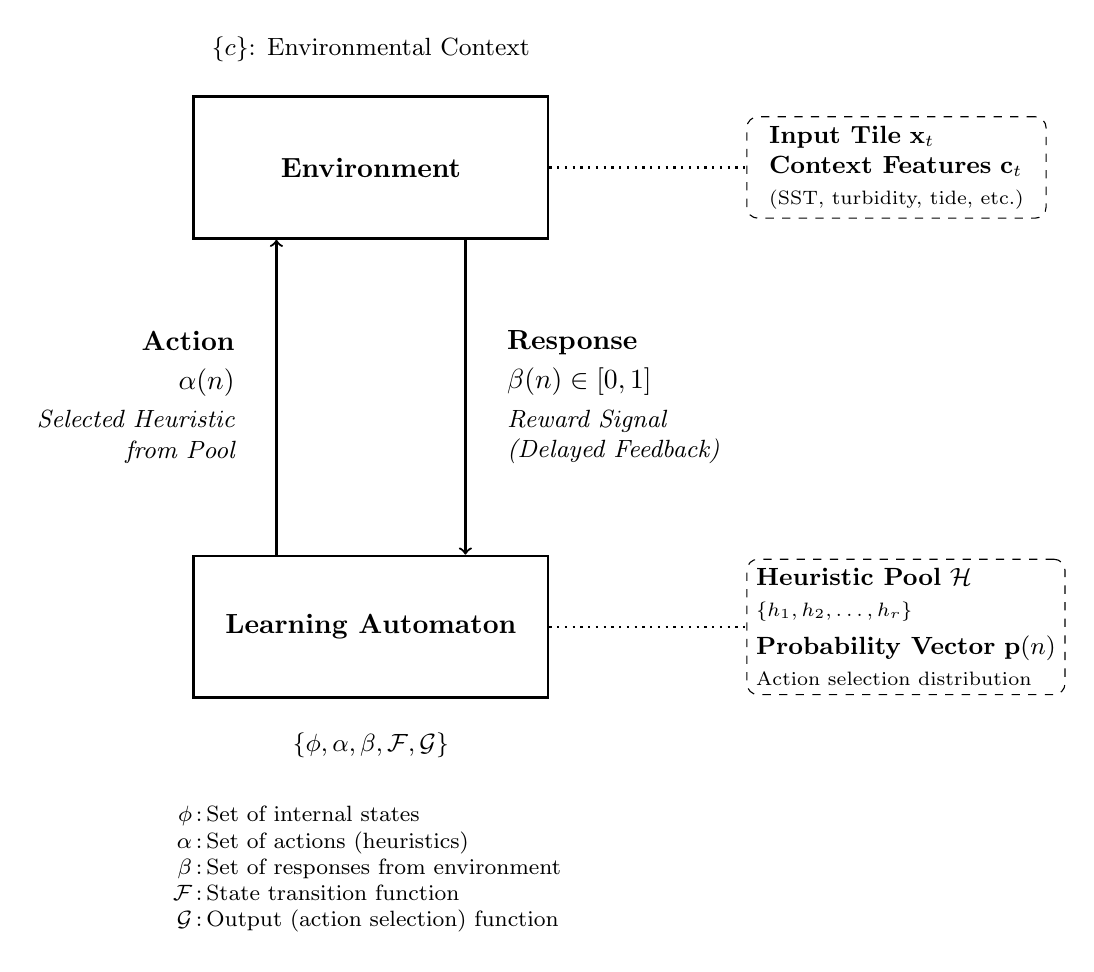
\begin{tikzpicture}[
        % Styles
        mainbox/.style={
            rectangle,
            draw=black,
            line width=1pt,
            minimum width=4.5cm,
            minimum height=1.8cm,
            align=center,
            font=\bfseries
        },
        label/.style={
            font=\small\itshape
        },
        tuple/.style={
            font=\small
        },
        arrow/.style={
            ->,
            thick,
            line width=0.8pt
        }
    ]

    % Environment Box
    \node[mainbox] (env) at (0, 0) {Environment};

    % Environment set notation above
    \node[tuple, above=0.3cm of env] {$\{c\}$: Environmental Context};

    % Environment description below the box
    \node[label, below=0.1cm of env, yshift=0.1cm] (env_desc) {};

    % Automaton Box
    \node[mainbox, below=4cm of env] (auto) {Learning Automaton};

    % Automaton tuple below
    \node[tuple, below=0.3cm of auto] {$\{\phi, \alpha, \beta, \mathcal{F}, \mathcal{G}\}$};

    % Left arrow: Action (Automaton to Environment)
    \draw[arrow] ([xshift=-1.2cm]auto.north) -- ([xshift=-1.2cm]env.south)
        node[midway, left=0.4cm, align=right] {
            \textbf{Action}\\[2pt]
            $\alpha(n)$\\[2pt]
            {\small\itshape Selected Heuristic}\\[-1pt]
            {\small\itshape from Pool}
        };

    % Right arrow: Response/Reward (Environment to Automaton)
    \draw[arrow] ([xshift=1.2cm]env.south) -- ([xshift=1.2cm]auto.north)
        node[midway, right=0.4cm, align=left] {
            \textbf{Response}\\[2pt]
            $\beta(n) \in [0,1]$\\[2pt]
            {\small\itshape Reward Signal}\\[-1pt]
            {\small\itshape (Delayed Feedback)}
        };

    % Component annotations on the right side
    \node[draw, dashed, rounded corners, minimum width=3.8cm, minimum height=1.2cm,
          right=2.5cm of env, align=left, font=\small] (env_detail) {
        \textbf{Input Tile} $\mathbf{x}_t$\\
        \textbf{Context Features} $\mathbf{c}_t$\\
        {\scriptsize (SST, turbidity, tide, etc.)}
    };
    \draw[dotted, thick] (env.east) -- (env_detail.west);

    \node[draw, dashed, rounded corners, minimum width=3.8cm, minimum height=1.6cm,
          right=2.5cm of auto, align=left, font=\small] (auto_detail) {
        \textbf{Heuristic Pool} $\mathcal{H}$\\
        {\scriptsize $\{h_1, h_2, \ldots, h_r\}$}\\[3pt]
        \textbf{Probability Vector} $\mathbf{p}(n)$\\
        {\scriptsize Action selection distribution}
    };
    \draw[dotted, thick] (auto.east) -- (auto_detail.west);

    % Legend/Key at the bottom
    \node[below=1.2cm of auto, xshift=0cm, align=left, font=\footnotesize] {
        \begin{tabular}{@{}r@{\,:\,}l@{}}
            $\phi$ & Set of internal states \\
            $\alpha$ & Set of actions (heuristics) \\
            $\beta$ & Set of responses from environment \\
            $\mathcal{F}$ & State transition function \\
            $\mathcal{G}$ & Output (action selection) function
        \end{tabular}
    };

    \end{tikzpicture}
    \caption{Learning Automata framework for adaptive kelp forest monitoring. The automaton selects detection heuristics $\alpha(n)$ from the pool based on the probability distribution $\mathbf{p}(n)$, applies them to the input tile within the environmental context, and updates its policy based on delayed reward signals $\beta(n)$.}
    \label{fig:framework-overview}
\end{figure}

\section{Problem Formulation}
\label{sec:problem-formulation}

Formally, we define the adaptive monitoring problem as follows:

\textbf{Input space:} Let $\mathbf{x}t \in \mathbb{R}^{B \times H \times W}$ be a tile of a satellite image at time $t$, where $B$ is the number of spectral bands, and $H \times W$ is the spatial resolution. Associated with each tile is a context vector $\mathbf{c}t \in \mathbb{R}^{D}$ encoding environmental conditions (e.g. sea surface temperature (SST), turbidity, solar geometry).

\textbf{Heuristic pool:} A pool of $r$ detection heuristics $\mathcal{H} = \{h1, h2, \ldots, hr\}$, where each heuristic $hi: \mathbf{x} \rightarrow \{0, 1\}^{H \times W}$ generates a binary segmentation map of kelp/non-kelp.

\textbf{Ground truth:} Validation labels $\mathbf{y}t \in \{0, 1\}^{H \times W}$ with label for time $t$ arriving eventually at time $t + \delta$ where $\delta$ varies from days to months.

\textbf{Performance metric:} A reward function R : ( hat {y}, y ) -> [0, 1] that measures the quality of detection, such as Intersection over Union (IoU) or F1-score.

\textbf{Objective:} Learn a policy $\pi:(\mathbf{x}, \mathbf{c})\to\Delta^{r-1}$ that takes inputs and context and outputs a probability distribution over heuristics such that the expected reward is maximized:
\begin{equation}
    \pi^* = \arg\max_\pi \mathbb{E}_{(\mathbf{x}, \mathbf{c}, \mathbf{y}) \sim \mathcal{D}} \left[ \sum_{i=1}^{r} \pi(\mathbf{x}, \mathbf{c})_i \cdot R(h_i(\mathbf{x}), \mathbf{y}) \right]
\end{equation}

\section{Learning Automata Framework Design}
\label{sec:la-framework}

\subsection{Component 1: Global Policy Learning}
\label{subsec:component1}

The global policy maintains a probability vector $\mathbf{p} = [p_1, p_2, \ldots, p_r]$ over the $r$ heuristics, which is updated by a modified Linear Reward-Inaction scheme.

\textbf{Initialization:} Uniform distribution $p_i(0) = 1/r$ for all $i$.

\textbf{Action selection:} At each time step, sample heuristic $h_i$ with probability $p_i$ (potentially modified by context-aware blending, see Section~\ref{subsec:component2}).

\textbf{Reward computation:} When validation label $\mathbf{y}_t$ arrives for a prediction made at time $t$ using heuristic $h_i$:
\begin{equation}
    R_t = \text{IoU}(h_i(\mathbf{x}_t), \mathbf{y}_t) = \frac{|h_i(\mathbf{x}_t) \cap \mathbf{y}_t|}{|h_i(\mathbf{x}_t) \cup \mathbf{y}_t|}
\end{equation}

\textbf{S-model environment:} Rather than binary P-model feedback, we use S-model (continuous) rewards where $R \in [0, 1]$. The update equations become:
\begin{align}
    p_i(n+1) &= p_i(n) + \lambda \cdot R \cdot [1 - p_i(n)] \\
    p_j(n+1) &= p_j(n) - \lambda \cdot R \cdot p_j(n), \quad j \neq i
\end{align}
where $\lambda \in (0, 1)$ is the learning rate. This maintains the L$_\text{R-I}$ property of only updating on positive feedback (when $R > 0$), scaled by reward magnitude.

\textbf{Multi-objective extension:} Beyond segmentation accuracy, the reward can incorporate additional objectives:
\begin{equation}
    R_\text{total} = w_1 \cdot R_\text{IoU} + w_2 \cdot R_\text{speed} + w_3 \cdot R_\text{uncertainty} + w_4 \cdot R_\text{carbon}
\end{equation}
where $R_\text{speed}$ rewards computational efficiency, $R_\text{uncertainty}$ rewards well-calibrated confidence, and $R_\text{carbon}$ penalizes computational carbon footprint. Weights $w_i$ can be set based on application priorities.

\subsection{Component 2: Context-Aware Local Adaptation}
\label{subsec:component2}

To enable generalization across the heterogeneous environmental conditions of BC's coastline, Component 2 implements context-dependent heuristic selection based on the principles of Generalized Learning Automata (GLA).

\textbf{Context feature extraction:} From each input tile and associated metadata, extract a $D$-dimensional context vector $\mathbf{c}$ encoding:
\begin{itemize}
    \item Spectral statistics (mean, variance of each band)
    \item Spatial texture features (entropy, homogeneity)
    \item Temporal context (day of year, time since last valid observation)
    \item Environmental conditions (SST from auxiliary data, tide height, solar zenith angle)
    \item Geographic location (latitude, longitude, distance to shore)
\end{itemize}

\textbf{Memory bank:} Maintain a memory bank $\mathcal{M} = \{(\mathbf{c}_j, \mathbf{p}_j, R_j)\}_{j=1}^{M}$ of past context vectors, associated local probability distributions, and observed rewards.

\textbf{k-NN retrieval:} For new context vector $\mathbf{c}$, fetch $k$ most similar entries from $\mathcal{M}$ using FAISS (Facebook AI Similarity Search) for efficient approximate nearest neighbor search:
\begin{equation}
    \mathcal{N}_k(\mathbf{c}) = \text{arg-}k\text{-min}_{\mathbf{c}_j \in \mathcal{M}} \|\mathbf{c} - \mathbf{c}_j\|_2
\end{equation}

\textbf{Local probability estimation:} Compute local heuristic preferences as the reward-weighted average of retrieved entries:
\begin{equation}
    \mathbf{p}_\text{local}(\mathbf{c}) = \frac{\sum_{j \in \mathcal{N}_k(\mathbf{c})} w_j \cdot R_j \cdot \mathbf{p}_j}{\sum_{j \in \mathcal{N}_k(\mathbf{c})} w_j \cdot R_j}
\end{equation}
where $w_j = \exp(-\|\mathbf{c} - \mathbf{c}_j\|_2^2 / \sigma^2)$ are distance-based weights.

\textbf{Global-local blending:} The final selection probability is a combination of the global and local estimates:
\begin{equation}
    \mathbf{p}_\text{final}(\mathbf{c}) = \alpha(\mathbf{c}) \cdot \mathbf{p}_\text{global} + (1 - \alpha(\mathbf{c})) \cdot \mathbf{p}_\text{local}(\mathbf{c})
\end{equation}
where $\alpha(\mathbf{c}) \in [0, 1]$ is an adaptive blending coefficient. When the memory bank contains few similar entries (low confidence in local estimate), $\alpha \rightarrow 1$ favors the global policy; when many similar entries exist with consistent performance, $\alpha \rightarrow 0$ favors local adaptation.

\subsection{Component 3: Sparse Label Handling}
\label{subsec:component3}

To deal with the asynchronous arrival of validation labels, Component 3 has a buffering and delayed reward propagation mechanism.

\textbf{Prediction buffer:} Maintain a FIFO buffer $\mathcal{B} = \{(t_j, \mathbf{x}_j, \mathbf{c}_j, i_j, \hat{\mathbf{y}}_j)\}$ for storing timestamps, inputs, contexts, selected heuristic indices, and predictions for tiles waiting to be validated.

\textbf{Hash map lookup:} Use a hash map $\mathcal{L}: \text{(location, time)} \rightarrow \text{buffer\_index}$ for O(1) lookup when validation labels arrive.

\textbf{Label arrival processing:} When validation label $\mathbf{y}$ arrives for location $\ell$ and time $t$:
\begin{enumerate}
    \item Look up entry in buffer using $\mathcal{L}(\ell, t)$
    \item Compute reward $R = \text{IoU}(\hat{\mathbf{y}}, \mathbf{y})$
    \item Update Component 1 global policy with $(i, R)$
    \item Update Component 2 memory bank with $(\mathbf{c}, \mathbf{p}_\text{final}, R)$
    \item Remove entry from buffer
\end{enumerate}

\textbf{Buffer management:} Entries older than a threshold $T_\text{max}$ (e.g., 6 months) are removed without update, under the assumption that conditions have changed too much for the reward to be informative.

\textbf{Temporal decay (optional):} Rewards for older predictions can be discounted:
\begin{equation}
    R_\text{effective} = R \cdot \gamma^{\delta}
\end{equation}
where $\delta = t_\text{label} - t_\text{prediction}$ is the delay in days and $\gamma < 1$ is a decay factor.

\section{Heuristic Pool Design}
\label{sec:heuristic-pool}

The heuristic pool contains 12 detection methods with three levels of complexity:

\subsection{Tier 1: Spectral Indices (4 heuristics)}

Simple, interpretable approaches from spectral band ratios:
\begin{enumerate}
    \item \textbf{NDVI threshold:} $\text{NDVI} = (B_\text{NIR} - B_\text{Red}) / (B_\text{NIR} + B_\text{Red}) > \tau_\text{NDVI}$
    \item \textbf{FAI threshold:} Floating Algae Index using red-edge bands $> \tau_\text{FAI}$
    \item \textbf{GNDVI threshold:} Green NDVI using green instead of red $> \tau_\text{GNDVI}$
    \item \textbf{Multi-index ensemble:} Majority vote of above 3 indices
\end{enumerate}

Thresholds $\tau$ can be fixed (based on literature) or learned as continuous actions via CARLA-type continuous automata \citep{Cuevas2011}.

\subsection{Tier 2: Classical Machine Learning (4 heuristics)}

Methods that combine the multiple features using learned decision boundaries:
\begin{enumerate}
    \setcounter{enumi}{4}
    \item \textbf{Random Forest:} 100-tree ensemble on spectral features, pre-trained on labeled BC data
    \item \textbf{Gradient Boosting:} XGBoost classifier on same features
    \item \textbf{SVM with RBF kernel:} Support vector machine with radial basis function kernel
    \item \textbf{K-means clustering:} Unsupervised clustering followed by class assignment based on spectral centroids
\end{enumerate}

\subsection{Tier 3: Deep Learning (4 heuristics)}

Neural network architectures for semantic segmentation:
\begin{enumerate}
    \setcounter{enumi}{8}
    \item \textbf{U-Net (basic):} Standard U-Net architecture with ResNet-18 encoder
    \item \textbf{U-Net (deep):} U-Net + ResNet-50 encoder, more parameters
    \item \textbf{DeepLab v3+:} Atrous spatial pyramid pooling for multi-scale context
    \item \textbf{Lightweight U-Net:} MobileNet encoder for fast inference
\end{enumerate}

Deep learning models are trained on the available labeled BC data beforehand and are fine-tuned on validation labels as they become available.

\section{Experimental Design}
\label{sec:experimental-design}

\subsection{Dataset: BC Bull Kelp}
\label{subsec:dataset}

\paragraph{Imagery:} Sentinel-2 Level-2A (surface reflectance) imagery tiles for BC coastal waters 2017--2024. Preprocessing includes:
\begin{itemize}
    \item Cloud/shadow masking using Scene Classification Layer
    \item Land masking using vector shoreline data
    \item Tile extraction at 256$\times$256 pixels (2.56 km$^2$ at 10m resolution)
    \item Band selection: B2 (blue), B3 (green), B4 (red), B5 (red-edge), B8 (NIR)
\end{itemize}

\paragraph{Labels:} Ground-truth kelp extent maps from:
\begin{itemize}
    \item ShoreZone oblique photography interpretations
    \item WorldView high-resolution classifications (where available)
    \item In-situ surveys from research partners
    \item Citizen science observations (iNaturalist, kelp-specific projects)
\end{itemize}

\paragraph{Environmental context:} Auxiliary data including:
\begin{itemize}
    \item Sea surface temperature from NOAA CoralTemp
    \item Tide height from CHS tidal predictions
    \item Ocean color products (chlorophyll, turbidity) from Sentinel-3 OLCI
\end{itemize}

\subsection{Evaluation Protocol}
\label{subsec:eval-protocol}

We design 3 evaluation protocols to evaluate different aspects of adaptation:

\paragraph{Protocol A: Temporal adaptation}
\begin{itemize}
    \item Train on 2017--2020 data
    \item Validate on 2021--2022 data
    \item Test on 2023--2024 data
    \item Evaluate performance over interannual variability
\end{itemize}

\paragraph{Protocol B: Spatial adaptation}
\begin{itemize}
    \item Train on subset of regions (e.g., southern Vancouver Island)
    \item Validate on held-out regions from same general area
    \item Test on separate regions (e.g. central coast, northern coast)
    \item Evaluate generalization along geographic and environmental gradients
\end{itemize}

\paragraph{Protocol C: Sparse label simulation}
\begin{itemize}
    \item Withhold varying fractions of labels (10\%, 50\%, 90\%)
    \item Introduce variable delay (1 day to 6 months)
    \item Measure learning efficiency as a function of label availability
\end{itemize}

\subsection{Evaluation Metrics}
\label{subsec:metrics}

\paragraph{Detection performance:}
\begin{itemize}
    \item Intersection over Union (IoU): $\frac{|P \cap G|}{|P \cup G|}$
    \item F1-score: $\frac{2 \cdot \text{Precision} \cdot \text{Recall}}{\text{Precision} + \text{Recall}}$
    \item Precision and Recall separately
    \item Area Under ROC Curve (AUC) for probabilistic outputs
\end{itemize}

\paragraph{Adaptation metrics:}
\begin{itemize}
    \item Regret: cumulative difference from oracle that always selects best heuristic
    \item Convergence rate: number of labels needed to achieve 90\% of asymptotic performance
    \item Stability: variance in heuristic selection probabilities over time
\end{itemize}

\paragraph{Computational efficiency:}
\begin{itemize}
    \item Inference time per tile
    \item Memory footprint
    \item Carbon cost estimation via CodeCarbon
\end{itemize}

\subsection{Ablation Studies}
\label{subsec:ablation}

Systematic ablations to understand component contributions:

\begin{enumerate}
    \item \textbf{Without Component 2:} Use only global policy, no context-aware adaptation
    \item \textbf{Without Component 3:} Assume immediate labels, no delayed reward handling
    \item \textbf{Without pursuit/estimator extensions:} Basic L$_\text{R-I}$ only
    \item \textbf{Heuristic pool ablations:} Remove each tier to assess contribution
    \item \textbf{Context feature ablations:} Subset of context features to identify most informative
\end{enumerate}

\section{Conceptual Models for Research Questions}
\label{sec:conceptual-models}

\subsection{RQ1 Conceptual Model: Adaptation with Limited Labels}
\label{subsec:rq1-model}

\textbf{Hypothesis:} The L$_\text{R-I}$ learning automata scheme can achieve effective adaptation using 10-100$\times$ fewer labels than supervised approaches.

\textbf{Mechanism:} Unlike supervised learning which requires dense labels to estimate gradients, L$_\text{R-I}$ only needs sparse binary/continuous feedback to shift probability mass toward better-performing heuristics. The ``inaction'' property means missing labels simply leave probabilities unchanged, gracefully handling sparse feedback. Figure~\ref{fig:rq1-model} illustrates this mechanism.

\textbf{Validation:} Compare label efficiency curves (performance vs.\ number of labels) between:
\begin{itemize}
    \item Proposed LA framework
    \item Supervised CNN with varying training set sizes
    \item Online learning baseline with random updates when labels missing
\end{itemize}

\begin{figure}[H]
    \centering
    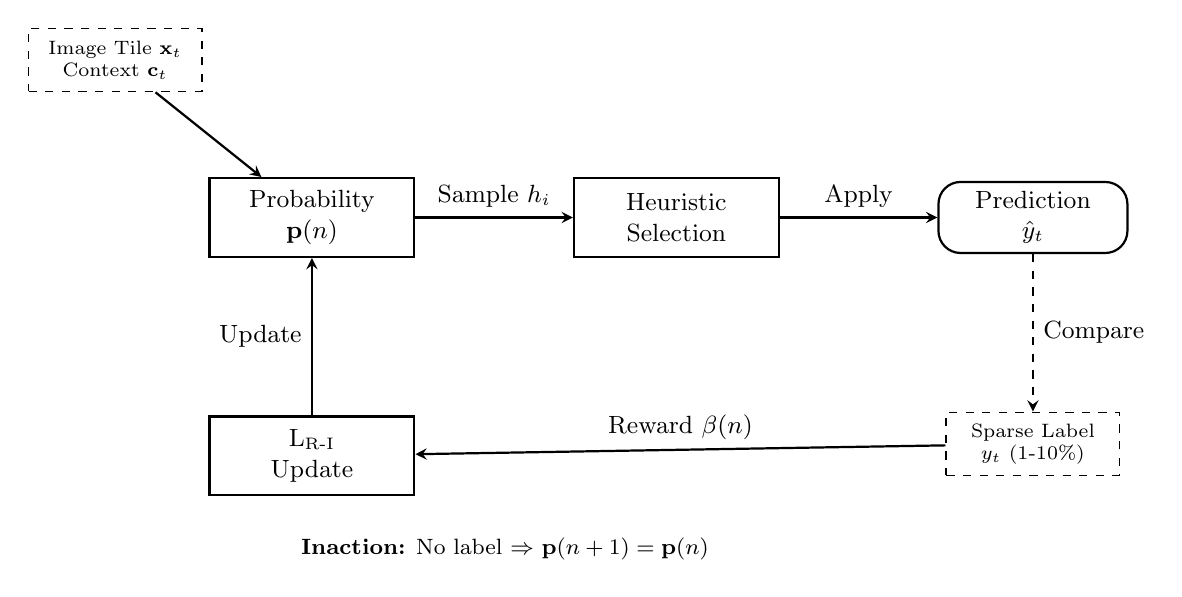
\begin{tikzpicture}[
        box/.style={rectangle, draw=black, line width=0.8pt, minimum width=2.6cm, minimum height=1cm, align=center, font=\small},
        roundbox/.style={rectangle, draw=black, line width=0.8pt, rounded corners=8pt, minimum width=2.4cm, minimum height=0.9cm, align=center, font=\small},
        inputbox/.style={rectangle, draw=black, line width=0.6pt, dashed, minimum width=2.2cm, minimum height=0.8cm, align=center, font=\scriptsize},
        arrow/.style={->, thick, >=stealth},
        dasharrow/.style={->, thick, >=stealth, dashed}
    ]

    % Input: Image Tile + Context
    \node[inputbox] (input) at (-2.5, 2) {Image Tile $\mathbf{x}_t$\\Context $\mathbf{c}_t$};

    % Probability Distribution
    \node[box] (prob) at (0,0) {Probability\\$\mathbf{p}(n)$};

    % Heuristic Selection
    \node[box, right=2cm of prob] (select) {Heuristic\\Selection};

    % Prediction Output
    \node[roundbox, right=2cm of select] (pred) {Prediction\\$\hat{y}_t$};

    % Sparse Label (may or may not arrive)
    \node[inputbox, below=2cm of pred] (label) {Sparse Label\\$y_t$ (1-10\%)};

    % LA Update
    \node[box, below=2cm of prob] (la) {L$_\text{R-I}$\\Update};

    % Arrows - main flow
    \draw[arrow] (input) -- (prob);
    \draw[arrow] (prob) -- node[above, font=\small] {Sample $h_i$} (select);
    \draw[arrow] (select) -- node[above, font=\small] {Apply} (pred);

    % Arrow from label to LA (reward calculation)
    \draw[arrow] (label) -- node[above, font=\small] {Reward $\beta(n)$} (la);

    % Arrow from LA back to probability
    \draw[arrow] (la) -- node[left, font=\small] {Update} (prob);

    % Dashed arrow showing prediction goes to validation
    \draw[dasharrow] (pred) -- node[right, font=\small] {Compare} (label);

    % Inaction annotation - positioned below the bottom row
    \node[below=0.4cm of la, xshift=2.5cm, align=center, font=\footnotesize] (inaction) {
        \textbf{Inaction:} No label $\Rightarrow$ $\mathbf{p}(n+1) = \mathbf{p}(n)$
    };

    \end{tikzpicture}
    \caption{\textbf{RQ1 Conceptual Model:} Given an input satellite tile $\mathbf{x}_t$ with environmental context $\mathbf{c}_t$, a detection heuristic is sampled from the probability distribution $\mathbf{p}(n)$ and applied to produce a kelp prediction $\hat{y}_t$. When a sparse validation label $y_t$ arrives (typically 1--10\% of predictions), the reward signal $\beta(n)$ triggers an L$_\text{R-I}$ update that shifts probability mass toward successful heuristics. Critically, when no label is available, which is the common case, the \emph{inaction property} ensures $\mathbf{p}$ remains unchanged, enabling stable learning from sparse feedback.}
    \label{fig:rq1-model}
\end{figure}

\subsection{RQ2 Conceptual Model: Heterogeneous Region Coverage}
\label{subsec:rq2-model}

\textbf{Hypothesis:} Adaptive heuristic selection achieves better coverage across environmental conditions than any fixed method.

\textbf{Mechanism:} There is a complementarity between different heuristics failure modes. Spectral indices do not work under turbid conditions but are robust to atmospheric variation; deep learning models capture complex patterns but can overfit to training distribution. The LA framework learns to select the right tool for each context, as shown in Figure~\ref{fig:rq2-model}.

\textbf{Validation:} Stratify test set by environmental conditions (e.g., turbidity quartiles, SST ranges) and compare:
\begin{itemize}
    \item LA framework performance across strata
    \item Best single heuristic performance across strata
    \item Oracle (best per-stratum heuristic) as upper bound
\end{itemize}

\begin{figure}[H]
    \centering
    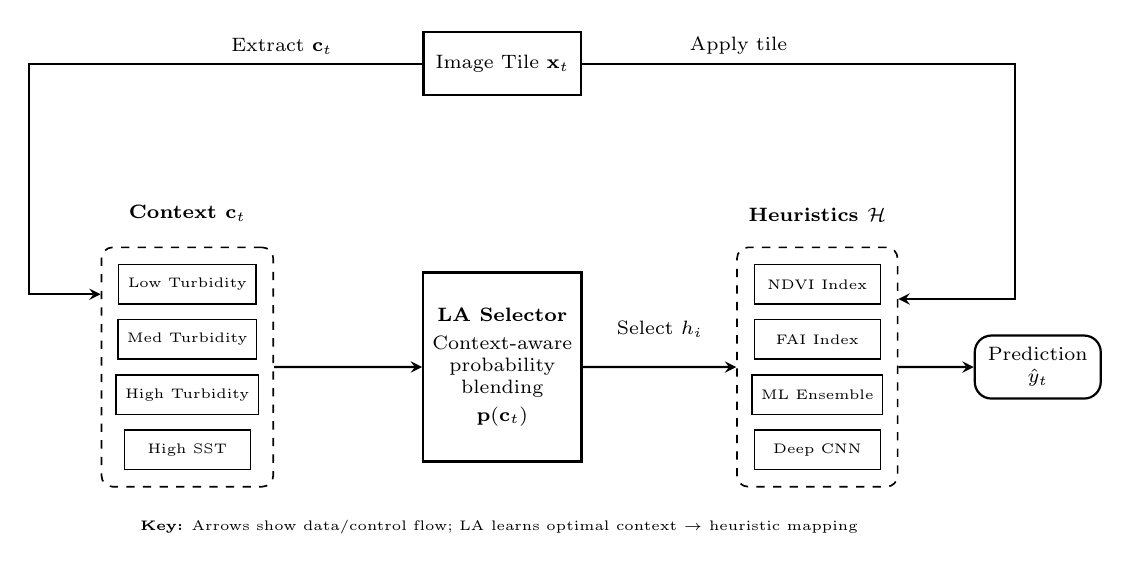
\begin{tikzpicture}[
        box/.style={rectangle, draw=black, line width=0.8pt, minimum width=2cm, minimum height=0.7cm, align=center, font=\scriptsize},
        smallbox/.style={rectangle, draw=black, line width=0.5pt, minimum width=1.6cm, minimum height=0.5cm, align=center, font=\tiny},
        inputbox/.style={rectangle, draw=black, line width=0.8pt, minimum width=2cm, minimum height=0.8cm, align=center, font=\scriptsize},
        outputbox/.style={rectangle, draw=black, line width=0.8pt, rounded corners=6pt, minimum width=1.6cm, minimum height=0.8cm, align=center, font=\scriptsize},
        groupbox/.style={rectangle, draw=black, line width=0.6pt, dashed, rounded corners=4pt},
        arrow/.style={->, thick, >=stealth}
    ]

    % Input: Satellite Tile (center top)
    \node[inputbox] (input) at (4, 3.5) {Image Tile $\mathbf{x}_t$};

    % === Context Group (left side) ===
    \node[smallbox] (cond1) at (0, 0.7) {Low Turbidity};
    \node[smallbox] (cond2) at (0, 0) {Med Turbidity};
    \node[smallbox] (cond3) at (0, -0.7) {High Turbidity};
    \node[smallbox] (cond4) at (0, -1.4) {High SST};

    % Dashed box around contexts
    \node[groupbox, fit=(cond1)(cond4), inner sep=6pt] (contextbox) {};
    \node[above=0.2cm of contextbox, font=\scriptsize\bfseries] {Context $\mathbf{c}_t$};

    % === LA Selector (center) ===
    \node[box, minimum height=2.4cm, minimum width=2cm] (la) at (4, -0.35) {
        \textbf{LA Selector}\\[2pt]
        Context-aware\\
        probability\\
        blending\\[2pt]
        $\mathbf{p}(\mathbf{c}_t)$
    };

    % === Heuristics Group (right side) ===
    \node[smallbox] (h1) at (8, 0.7) {NDVI Index};
    \node[smallbox] (h2) at (8, 0) {FAI Index};
    \node[smallbox] (h3) at (8, -0.7) {ML Ensemble};
    \node[smallbox] (h4) at (8, -1.4) {Deep CNN};

    % Dashed box around heuristics
    \node[groupbox, fit=(h1)(h4), inner sep=6pt] (heurbox) {};
    \node[above=0.2cm of heurbox, font=\scriptsize\bfseries] {Heuristics $\mathcal{H}$};

    % === Output: Prediction ===
    \node[outputbox] (output) at (10.8, -0.35) {Prediction\\$\hat{y}_t$};

    % === Arrows with proper text placement ===

    % Arrow from Input LEFT: goes left beyond Context box, down, then right into west side
    \draw[arrow] (input.west) -- ++(-5,0) |- (contextbox.140);
    \node[font=\scriptsize, above] at (1.2, 3.5) {Extract $\mathbf{c}_t$};

    % Arrow from Input RIGHT: goes right beyond Heuristics box, down, then left into east side
    \draw[arrow] (input.east) -- ++(5.5,0) |- (heurbox.40);
    \node[font=\scriptsize, above] at (7, 3.5) {Apply tile};

    % Arrow from Context box to LA Selector
    \draw[arrow] (contextbox.east) -- (la.west);

    % Arrow from LA Selector to Heuristics box
    \draw[arrow] (la.east) -- (heurbox.west);
    \node[font=\scriptsize, above] at (6, -0.1) {Select $h_i$};

    % Arrow from Heuristics box to Prediction
    \draw[arrow] (heurbox.east) -- (output.west);

    % Annotation
    \node[below=0.6cm of la, align=center, font=\tiny] {
        \textbf{Key:} Arrows show data/control flow; LA learns optimal context $\rightarrow$ heuristic mapping
    };

    \end{tikzpicture}
    \caption{\textbf{RQ2 Conceptual Model:} Given a satellite tile $\mathbf{x}_t$, two parallel paths proceed: (1) environmental context $\mathbf{c}_t$ is extracted and sent to the LA Selector (left path), and (2) the tile is routed to the heuristic pool for processing (right path). The LA Selector uses the context to compute a probability distribution $\mathbf{p}(\mathbf{c}_t)$ and selects heuristic $h_i$, which then processes the tile to produce prediction $\hat{y}_t$. Arrows indicate data and control flow direction. Different heuristics have complementary failure modes: spectral indices (NDVI, FAI) excel under clear water; ML/deep learning models handle complex patterns. The LA learns which heuristics perform best for each environmental condition.}
    \label{fig:rq2-model}
\end{figure}

\subsection{RQ3 Conceptual Model: Sparse Label Learning}
\label{subsec:rq3-model}

\textbf{Hypothesis:} The buffering and delayed reward propagation mechanism enables effective learning despite asynchronous feedback.

\textbf{Mechanism:} By storing predictions until labels arrive, the system can provide accurate reward signals regardless of delay. The temporal decay term downweights very old feedback that may no longer be relevant due to environmental change. This process is depicted in Figure~\ref{fig:rq3-model}.

\textbf{Validation:} Simulate different delay distributions and compare:
\begin{itemize}
    \item LA framework learning curves
    \item Baseline that discards delayed feedback
    \item Baseline that treats delayed feedback as immediate
\end{itemize}

\begin{figure}[H]
    \centering
    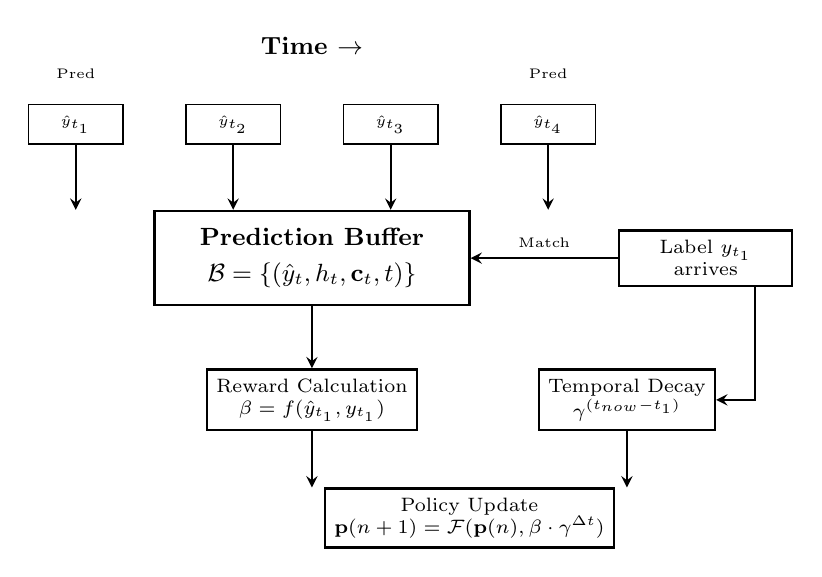
\begin{tikzpicture}[
        box/.style={rectangle, draw=black, line width=0.8pt, minimum width=2cm, minimum height=0.7cm, align=center, font=\scriptsize},
        timeline/.style={rectangle, draw=black, line width=0.6pt, minimum width=1.2cm, minimum height=0.5cm, align=center, font=\tiny},
        buffer/.style={rectangle, draw=black, line width=0.8pt, minimum width=4cm, minimum height=1.2cm, align=center, font=\small},
        arrow/.style={->, thick, >=stealth},
        dasharrow/.style={->, dashed, thick, >=stealth}
    ]

    % Timeline at top
    \node[font=\small\bfseries] at (0, 3) {Time $\rightarrow$};

    % Prediction nodes
    \node[timeline] (p1) at (-3, 2) {$\hat{y}_{t_1}$};
    \node[timeline] (p2) at (-1, 2) {$\hat{y}_{t_2}$};
    \node[timeline] (p3) at (1, 2) {$\hat{y}_{t_3}$};
    \node[timeline] (p4) at (3, 2) {$\hat{y}_{t_4}$};

    \node[above=0.2cm of p1, font=\tiny] {Pred};
    \node[above=0.2cm of p4, font=\tiny] {Pred};

    % Prediction Buffer
    \node[buffer] (buf) at (0, 0.3) {
        \textbf{Prediction Buffer}\\[2pt]
        $\mathcal{B} = \{(\hat{y}_t, h_t, \mathbf{c}_t, t)\}$
    };

    % Arrows to buffer
    \draw[arrow] (p1.south) -- (buf.north -| p1);
    \draw[arrow] (p2.south) -- (buf.north -| p2);
    \draw[arrow] (p3.south) -- (buf.north -| p3);
    \draw[arrow] (p4.south) -- (buf.north -| p4);

    % Delayed label arrival
    \node[box, minimum width=2.2cm] (label) at (5, 0.3) {Label $y_{t_1}$\\arrives};

    % Arrow from label to buffer lookup
    \draw[arrow] (label.west) -- node[above, font=\tiny] {Match} (buf.east);

    % Reward calculation
    \node[box, minimum width=2.5cm] (reward) at (0, -1.5) {Reward Calculation\\$\beta = f(\hat{y}_{t_1}, y_{t_1})$};

    \draw[arrow] (buf.south) -- (reward.north);

    % Temporal decay
    \node[box, minimum width=2.2cm] (decay) at (4, -1.5) {Temporal Decay\\$\gamma^{(t_{now} - t_1)}$};

    \draw[arrow] (label.330) |- (decay.east);

    % Policy update
    \node[box, minimum width=3cm] (update) at (2, -3) {Policy Update\\$\mathbf{p}(n+1) = \mathcal{F}(\mathbf{p}(n), \beta \cdot \gamma^{\Delta t})$};

    \draw[arrow] (reward.south) -- ++(0,-0.3) -| (update.north -| reward);
    \draw[arrow] (decay.south) -- ++(0,-0.3) -| (update.north -| decay);

    \end{tikzpicture}
    \caption{\textbf{RQ3 Conceptual Model:} The sparse label learning process proceeds as follows: (1) Predictions $\hat{y}_t$ are generated at various time points and stored in the prediction buffer $\mathcal{B}$ along with the selected heuristic $h_t$, context $\mathbf{c}_t$, and timestamp. (2) When a ground-truth label $y_{t_1}$ arrives (possibly after significant delay), the system matches it to the corresponding buffered prediction. (3) A reward signal $\beta$ is calculated by comparing the prediction to the label. (4) A temporal decay factor $\gamma^{\Delta t}$ is computed based on the time elapsed since the original prediction, downweighting stale feedback that may no longer reflect current conditions. (5) Both the reward and decay factor feed into the policy update, adjusting action probabilities $\mathbf{p}$ to improve future heuristic selection.}
    \label{fig:rq3-model}
\end{figure}

\subsection{RQ4 Conceptual Model: Indigenous Knowledge Integration}
\label{subsec:rq4-model}

\textbf{Hypothesis:} TEK can enhance automated monitoring through (a) historical baseline provision, (b) identification of culturally significant sites for prioritized monitoring, and (c) validation of automated detections using traditional observation.

\textbf{Mechanism:} Integration occurs through partnership with coastal First Nations, with specific protocols developed collaboratively. Potential integration points include:
\begin{itemize}
    \item TEK-derived site importance weights for evaluation metrics
    \item Traditional seasonal calendars informing temporal analysis
    \item Elder validation of ambiguous automated detections
\end{itemize}
The integration framework is illustrated in Figure~\ref{fig:rq4-model}.

\textbf{Validation:} Qualitative assessment through community feedback; quantitative assessment through comparison of TEK-weighted vs.\ uniform metrics.

\begin{figure}[H]
    \centering
    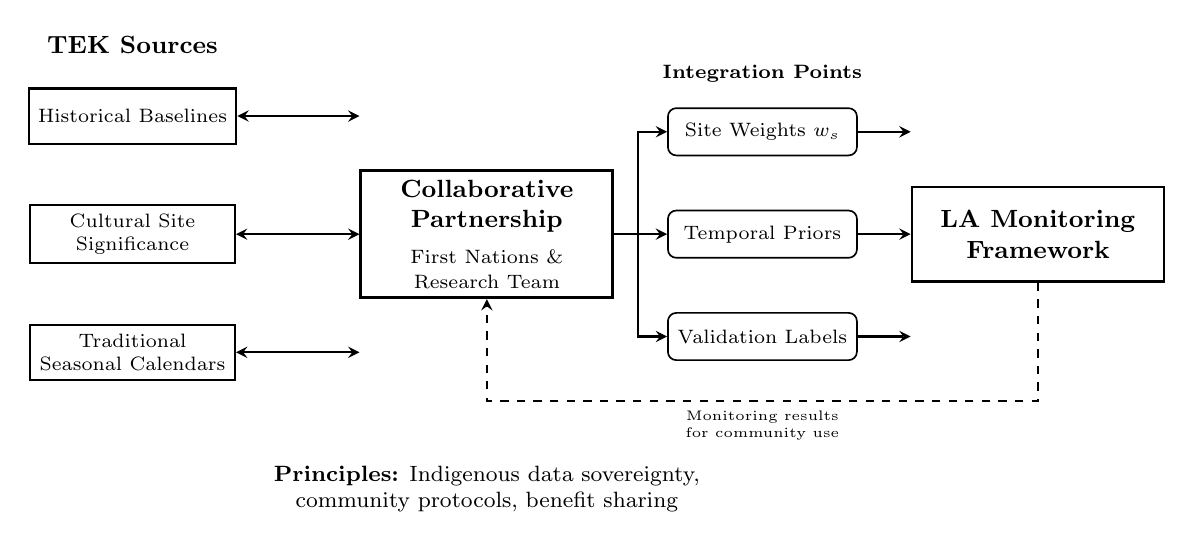
\begin{tikzpicture}[
        mainbox/.style={rectangle, draw=black, line width=1pt, minimum width=3.2cm, minimum height=1.2cm, align=center, font=\small},
        subbox/.style={rectangle, draw=black, line width=0.6pt, rounded corners=3pt, minimum width=2.4cm, minimum height=0.6cm, align=center, font=\scriptsize},
        tekbox/.style={rectangle, draw=black, line width=0.8pt, minimum width=2.6cm, minimum height=0.7cm, align=center, font=\scriptsize},
        arrow/.style={->, thick, >=stealth},
        doublearrow/.style={<->, thick, >=stealth},
        note/.style={font=\tiny\itshape}
    ]

    % Central Partnership Node
    \node[mainbox] (partner) at (0, 0) {
        \textbf{Collaborative}\\
        \textbf{Partnership}\\[2pt]
        {\scriptsize First Nations \&}\\[-2pt]
        {\scriptsize Research Team}
    };

    % TEK Sources (left side)
    \node[tekbox] (tek1) at (-4.5, 1.5) {Historical Baselines};
    \node[tekbox] (tek2) at (-4.5, 0) {Cultural Site\\Significance};
    \node[tekbox] (tek3) at (-4.5, -1.5) {Traditional\\Seasonal Calendars};

    \node[above=0.3cm of tek1, font=\small\bfseries] {TEK Sources};

    % Automated System (right side)
    \node[mainbox] (auto) at (7, 0) {
        \textbf{LA Monitoring}\\
        \textbf{Framework}
    };

    % Integration Points (between partnership and automated)
    \node[subbox] (int1) at (3.5, 1.3) {Site Weights $w_s$};
    \node[subbox] (int2) at (3.5, 0) {Temporal Priors};
    \node[subbox] (int3) at (3.5, -1.3) {Validation Labels};

    \node[above=0.2cm of int1, font=\scriptsize\bfseries] {Integration Points};

    % Arrows from TEK to Partnership (bidirectional for respect)
    \draw[doublearrow] (tek1.east) -- (partner.west |- tek1);
    \draw[doublearrow] (tek2.east) -- (partner.west);
    \draw[doublearrow] (tek3.east) -- (partner.west |- tek3);

    % Arrows from Partnership to Integration Points
    \draw[arrow] (partner.east) -- ++(0.3,0) |- (int1.west);
    \draw[arrow] (partner.east) -- (int2.west);
    \draw[arrow] (partner.east) -- ++(0.3,0) |- (int3.west);

    % Arrows from Integration to Automated System
    \draw[arrow] (int1.east) -- (auto.west |- int1);
    \draw[arrow] (int2.east) -- (auto.west);
    \draw[arrow] (int3.east) -- (auto.west |- int3);

    % Benefits back to community
    \draw[arrow, dashed] (auto.south) -- ++(0,-1.5) -| node[below, pos=0.25, font=\tiny, align=center] {Monitoring results\\for community use} (partner.south);

    % Data Sovereignty annotation
    \node[below=2.0cm of partner, align=center, font=\footnotesize] {
        \textbf{Principles:} Indigenous data sovereignty,\\
        community protocols, benefit sharing
    };

    \end{tikzpicture}
    \caption{\textbf{RQ4 Conceptual Model:} The TEK integration process proceeds as follows: (1) Traditional Ecological Knowledge sources: historical baselines, cultural site significance, and seasonal calendars provide indigenous knowledge accumulated over generations. (2) This knowledge flows through a Collaborative Partnership between First Nations communities and the research team, with bidirectional arrows indicating mutual respect and co-design rather than extractive data collection. (3) The partnership transforms TEK into concrete integration points: site importance weights $w_s$ for prioritizing culturally significant areas, temporal priors from traditional calendars, and validation labels from elder observations. (4) These integration points feed into the LA Monitoring Framework to enhance kelp detection accuracy. (5) Monitoring results flow back to the community (dashed arrow), ensuring benefit sharing. All interactions are governed by indigenous data sovereignty principles and community-defined protocols.}
    \label{fig:rq4-model}
\end{figure}

\section{Indigenous Knowledge Integration Protocol}
\label{sec:tek-protocol}

Respectful integration of Traditional Ecological Knowledge requires careful consideration of indigenous data sovereignty and community protocols. We propose a phased approach:

\paragraph{Phase 1: Relationship building}
\begin{itemize}
    \item Establish relations with coastal First Nations communities through proper channels
    \item Introduce research goals and solicit feedback on relevance to community priorities
    \item Understand protocols for sharing knowledge within the community
\end{itemize}

\paragraph{Phase 2: Co-design}
\begin{itemize}
    \item Together identify possible integration points
    \item Develop data governance agreements that ensure community control
    \item Design mechanisms for sharing benefits
\end{itemize}

\paragraph{Phase 3: Implementation}
\begin{itemize}
    \item Integrate agreed-upon TEK elements into framework
    \item Maintain ongoing community engagement and feedback
    \item Ensure attribution and acknowledgment in all outputs
\end{itemize}

\paragraph{Phase 4: Evaluation and iteration}
\begin{itemize}
    \item Community led evaluation of integration success
    \item Iterative refinement based on feedback
    \item Documentation of process for replication in other contexts
\end{itemize}

This protocol recognizes that TEK integration is not a technical problem to be solved but a relational process to be nurtured.


% ============================================================================
% CHAPTER 4: EXPECTED RESULTS AND CONTRIBUTIONS
% ============================================================================
\chapter{Expected Results and Contributions}
\label{ch:contributions}

\section{Scientific Contributions}
\label{sec:scientific-contributions}

This research is expected to have the following scientific contributions:

\textbf{Novel application of learning automata to environmental monitoring:} Although learning automata have been used to image segmentation \citep{Cuevas2011} and sensor placement \citep{BenZvi2018}, this work is the first for satellite-based ecosystem monitoring. The blend of context-aware adaptation with the GLA principles takes the theory of Learning Automata into a new domain.

\textbf{Empirical characterization of heuristic complementarity:} The experimental design will uncover which detection heuristics perform well under which environmental conditions, thus providing empirical evidence for (or against) the hypothesis that detection heuristics with diverse heuristic pools are better than specialized approaches.

\textbf{Understanding of sparse feedback learning dynamics:} The sparse label experiments will characterize how learning efficiency degrades with label scarcity and delay, informing both theoretical understanding and practical system design.

\section{Methodological Contributions}
\label{sec:methodological-contributions}

\textbf{Sparse label handling mechanism:} The buffering and delayed reward propagation mechanism provides a principled solution to a practical problem of many operational monitoring systems. The mechanism is sufficiently general to be applicable to other areas where asynchronous feedback is involved.

\textbf{Context-aware adaptation framework:} The combination of memory-based similarity matching with global-local probability blending offers a template for systems which must generalize across heterogeneous conditions with limited site-specific calibration.

\textbf{Multi-objective reward formulation:} The extension of LA to multi-objective rewards (accuracy + speed + uncertainty + carbon) addresses increasing concerns about the environmental cost of machine learning, and the need for well-calibrated uncertainty.

\textbf{Evaluation protocols for adaptive systems:} The temporal, spatial and sparse label evaluation protocols can be used as benchmarks for future adaptive monitoring studies.

\section{Practical Applications}
\label{sec:practical-applications}

\textbf{Kelp forest conservation in BC:} An operational monitoring system based on this research could provide:
\begin{itemize}
    \item Coastline-scale kelp extent maps updated weekly to monthly
    \item Early warning of kelp forest decline in monitored areas
    \item Quantitative monitoring of recovery after disturbance
    \item Prioritization of areas for field survey or intervention
    \item Data to inform site selection for kelp restoration efforts as demonstrated by the decision framework of \citet{GiraldoOspina2024}
\end{itemize}

\textbf{Decision support for fisheries management:} Kelp forests provide juvenile fish habitat; kelp extent information could be used to make fisheries management decisions for herring, rockfish and other species.

\textbf{Climate change impact assessment:} Long-term kelp monitoring provides indicator data for the assessment of climate change impacts on temperate marine ecosystems.

\textbf{Blue carbon accounting:} Kelp forests sequester significant carbon; accurate extent mapping supports blue carbon initiatives and climate mitigation planning.

\textbf{Framework transferability:} The methodology developed for kelp monitoring should transfer to other spatially extensive, environmentally heterogeneous monitoring challenges, such as seagrass meadows, coral reefs, and terrestrial vegetation.


% ============================================================================
% CHAPTER 5: RESEARCH TIMELINE
% ============================================================================
\chapter{Research Timeline}
\label{ch:timeline}

\section{Phase 1: Foundation and Data Preparation}

\paragraph{Tasks:}
\begin{itemize}
    \item Complete literature review and refine methodology
    \item Acquire and preprocess Sentinel-2 imagery for BC coastal waters
    \item Compile ground-truth labels from available sources
    \item Implement baseline heuristics (Tier 1 spectral indices)
    \item Establish evaluation infrastructure
\end{itemize}

\section{Phase 2: Core Framework Development}

\paragraph{Tasks:}
\begin{itemize}
    \item Implement Component 1: Global Policy Learning with L$_\text{R-I}$
    \item Implement Component 2: Context-Aware Local Adaptation
    \item Implement Component 3: Sparse Label Handling
    \item Integrate components into unified framework
    \item Develop Tier 2 and Tier 3 heuristics
    \item Initial validation on subset of data
\end{itemize}

\section{Phase 3: Experimental Evaluation}

\paragraph{Tasks:}
\begin{itemize}
    \item Execute Protocol A: Experiments on temporal adaptation
    \item Execute Protocol B: Spatial adaptation experiments
    \item Execute Protocol C: Sparse label simulation
    \item Perform ablation studies
    \item Analyze results and refine methodology
\end{itemize}

\section{Phase 4: Extensions and Integration}

\paragraph{Tasks:}
\begin{itemize}
    \item Explore pursuit/estimator algorithm extensions
    \item Investigate multi-objective reward formulations
    \item Initiate indigenous knowledge integration (Phase 1 relationship building)
    \item Develop visualization and interpretation tools
\end{itemize}

\section{Phase 5: Thesis Completion}

\paragraph{Tasks:}
\begin{itemize}
    \item Synthesize results across experiments
    \item Write thesis chapters
    \item Prepare publications for journal submission
    \item Thesis defense and revisions
\end{itemize}

\section{Milestones Summary}

\begin{table}[H]
\centering
\footnotesize
\begin{tabular}{lll}
\toprule
\textbf{Milestone} & \textbf{Deliverable} & \textbf{Dependencies} \\
\midrule
M1 & Dataset and baselines ready & None \\
M2 & Core framework functional & M1 \\
M3 & Temporal experiments complete & M2 \\
M4 & Spatial experiments complete & M3 \\
M5 & Sparse label experiments complete & M3 \\
M6 & Extensions implemented & M4, M5 \\
M7 & Thesis draft complete & M6 \\
M8 & Thesis defense & M7 \\
\bottomrule
\end{tabular}
\caption{Research milestones and dependencies.}
\label{tab:milestones}
\end{table}


% ============================================================================
% REFERENCES
% ============================================================================
\bibliographystyle{apalike}
\bibliography{references}

\end{document}
